\documentclass[aos,preprint]{imsart}
\usepackage{xr}
	\externaldocument{./suppl}

%% Packages
\def\shownotes{0}
%\usepackage{natbib}
%\setcitestyle{authoryear,open={(},close={)}}
%\renewcommand{\cite}{\citep}
\usepackage[export]{adjustbox}
%\usepackage[margin=1in]{geometry}
%\usepackage{fullpage}
\usepackage{subfloat}
\usepackage[T1]{fontenc}    % use 8-bit T1 fonts
\usepackage{nicefrac}       % compact symbols for 1/2, etc.
\usepackage{microtype}      % microtypography
\usepackage{graphicx}
\usepackage[hidelinks]{hyperref}
\usepackage{macro_math}
\usepackage{macro_fan}
\usepackage{stmaryrd}
\usepackage{multirow}
\usepackage[us,12hr]{datetime}
\usepackage[utf8]{inputenc} % allow utf-8 input
\usepackage{caption,subcaption}
%\usepackage{breqn}

\usepackage{dsfont}


\newcommand*\samethanks[1][\value{footnote}]{\footnotemark[#1]}

%%%%%%%%%%%%%%%%%%%%%%%%%%%%%%%%%%%%%%%%%%%%%%
%%                                          %%
%% Uncomment next line to change            %%
%% the type of equation numbering           %%
%%                                          %%
%%%%%%%%%%%%%%%%%%%%%%%%%%%%%%%%%%%%%%%%%%%%%%
%\numberwithin{equation}{section}
%%%%%%%%%%%%%%%%%%%%%%%%%%%%%%%%%%%%%%%%%%%%%%
%%                                          %%
%% For Axiom, Claim, Corollary, Hypothezis, %%
%% Lemma, Theorem, Proposition              %%
%% use \theoremstyle{plain}                 %%
%%                                          %%
%%%%%%%%%%%%%%%%%%%%%%%%%%%%%%%%%%%%%%%%%%%%%%
%\theoremstyle{plain}

%%%%%%%%%%%%%%%%%%%%%%%%%%%%%%%%%%%%%%%%%%%%%%
%%                                          %%
%% For Assumption, Definition, Example,     %%
%% Notation, Property, Remark, Fact         %%
%% use \theoremstyle{remark}                %%
%%                                          %%
%%%%%%%%%%%%%%%%%%%%%%%%%%%%%%%%%%%%%%%%%%%%%%

%%%%%%%%%%%%%%%%%%%%%%%%%%%%%%%%%%%%%%%%%%%%%%
%% Please put your definitions here:        %%
%%%%%%%%%%%%%%%%%%%%%%%%%%%%%%%%%%%%%%%%%%%%%%

\endlocaldefs

\begin{document}

\begin{frontmatter}
%\title{High-dimensional Asymptotics of Linear Regression with Different Covariates and Sample Sizes}
%\title{A sample article title with some additional note\thanksref{t1}}

\title{High-dimensional Asymptotics of Transfer Learning for Linear Regression} 
%with Different Covariates and Sample Sizes}

\runtitle{Linear Regression with Different Covariates and Sample Sizes}
%\thankstext{T1}{A sample additional note to the title.}

\begin{aug}
%%%%%%%%%%%%%%%%%%%%%%%%%%%%%%%%%%%%%%%%%%%%%%
%%Only one address is permitted per author. %%
%%Only division, organization and e-mail is %%
%%included in the address.                  %%
%%Additional information can be included in %%
%%the Acknowledgments section if necessary. %%
%%%%%%%%%%%%%%%%%%%%%%%%%%%%%%%%%%%%%%%%%%%%%%
\author[A]{\fnms{Fan} \snm{Yang}\ead[label=e1]{fyang75@wharton.upenn.edu}}
\author[B]{\fnms{Hongyang R.} \snm{Zhang}\ead[label=e2,mark]{hrzhang@northeastern.edu}}
\author[C]{\fnms{Sen} \snm{Wu}\ead[label=e3,mark]{senwu@stanford.edu}} 
\author[A]{\fnms{Weijie J.} \snm{Su}\ead[label=e4,mark]{suw@wharton.upenn.edu} }
\and
\author[C]{\fnms{Christopher} \snm{R\'e}\ead[label=e5,mark]{chrismre@cs.stanford.edu}} 
%%%%%%%%%%%%%%%%%%%%%%%%%%%%%%%%%%%%%%%%%%%%%%
%% Addresses                                %%
%%%%%%%%%%%%%%%%%%%%%%%%%%%%%%%%%%%%%%%%%%%%%%
\address[A]{Department of Statistics,
University of Pennsylvania,
\printead{e1,e4}}
\address[B]{Khoury College of Computer Sciences, Northeastern University,
\printead{e2}}
\address[C]{Department of Computer Science, Stanford University,
\printead{e3,e5}}

\end{aug}

\begin{abstract}
	{\cor rewrite} Hard parameter sharing for multi-task learning is widely used in empirical research despite the fact that its generalization properties have not been well established in many cases. This paper studies its generalization properties in a fundamental setting: How does hard parameter sharing work given multiple linear regression tasks? We develop new techniques and establish a number of new results in the high-dimensional setting, where the sample size and feature dimension increase at a fixed ratio. First, we show a sharp bias-variance decomposition of hard parameter sharing, given multiple tasks with the same features. Second, we characterize the asymptotic bias-variance limit for two tasks, even when they have arbitrarily different sample size ratios and covariate shifts. We also demonstrate that these limiting estimates for the empirical loss are incredibly accurate in moderate dimensions. Finally, we explain an intriguing phenomenon where increasing one task's sample size helps another task initially by reducing variance but hurts eventually due to increasing bias. This suggests progressively adding data for optimizing hard parameter sharing, and we validate its efficiency in text classification tasks.
\end{abstract}

\begin{keyword}[class=MSC2020]
\kwd[Primary ]{62J05}
\kwd{60B20}
\kwd[; secondary ]{62E20, 62H10}
\end{keyword}

\begin{keyword}
\kwd{Hard parameter sharing, high-dimensional linear regression, random matrix theory, sample covariance matrices}
\end{keyword}

\end{frontmatter}
%%%%%%%%%%%%%%%%%%%%%%%%%%%%%%%%%%%%%%%%%%%%%%
%% Please use \tableofcontents for articles %%
%% with 50 pages and more                   %%
%%%%%%%%%%%%%%%%%%%%%%%%%%%%%%%%%%%%%%%%%%%%%%
%\tableofcontents



\section{Introduction}\label{sec_introduction}

{\cor rewrite} Hard parameter sharing (HPS) for multi-task learning is widely used in empirical research and goes back to the seminal work of \cite{C97}.
Recent work has revived interests in this approach because it improves performance and reduces the cost of collecting labeled data \cite{R17}.
It is generally applied by sharing the feature layers between all tasks while keeping an output layer for every task.
Often, hard parameter sharing offers two critical advantages if successfully applied.
First, it reduces model parameters since all tasks use the same feature space.
Second, it reduces the amount of labeled data needed from each task by augmenting the entire training dataset.

Hard parameter sharing works as an inductive transfer mechanism and a regularizer that reduces overfitting, both of which have great intuitive appeal \cite{R17}.
For example, by restricting the shared space's size, HPS encourages information sharing among multiple tasks \cite{KD12}.
Another source of inductive bias comes from the tasks and depends on datasets' properties such as sample sizes and task covariances \cite{WZR20}.
However, how these dataset properties impact HPS has not been well established.
%It becomes increasingly important to understand HPS' formal generalization properties.
Part of the challenge may be that HPS' generalization performance depends intricately on the sample size ratios and covariate shifts between tasks, and is not amenable to standard concentration results.
Previous results based on Rademacher complexity or VC dimensions have considered cases where all tasks' sample sizes are equal to logarithmic factors of the feature dimension \cite{B00,MPR16}, and when all tasks' sample sizes increase simultaneously \cite{AZ05,M06}.
%For, the generalization error scales down as the sample sizes of all tasks increase, when applied to the multi-task setting \cite{B00,AZ05,M06,MPR16,WZR20}.

\begin{figure*}[!t]
	\begin{subfigure}[t]{0.5\textwidth}
		\centering
		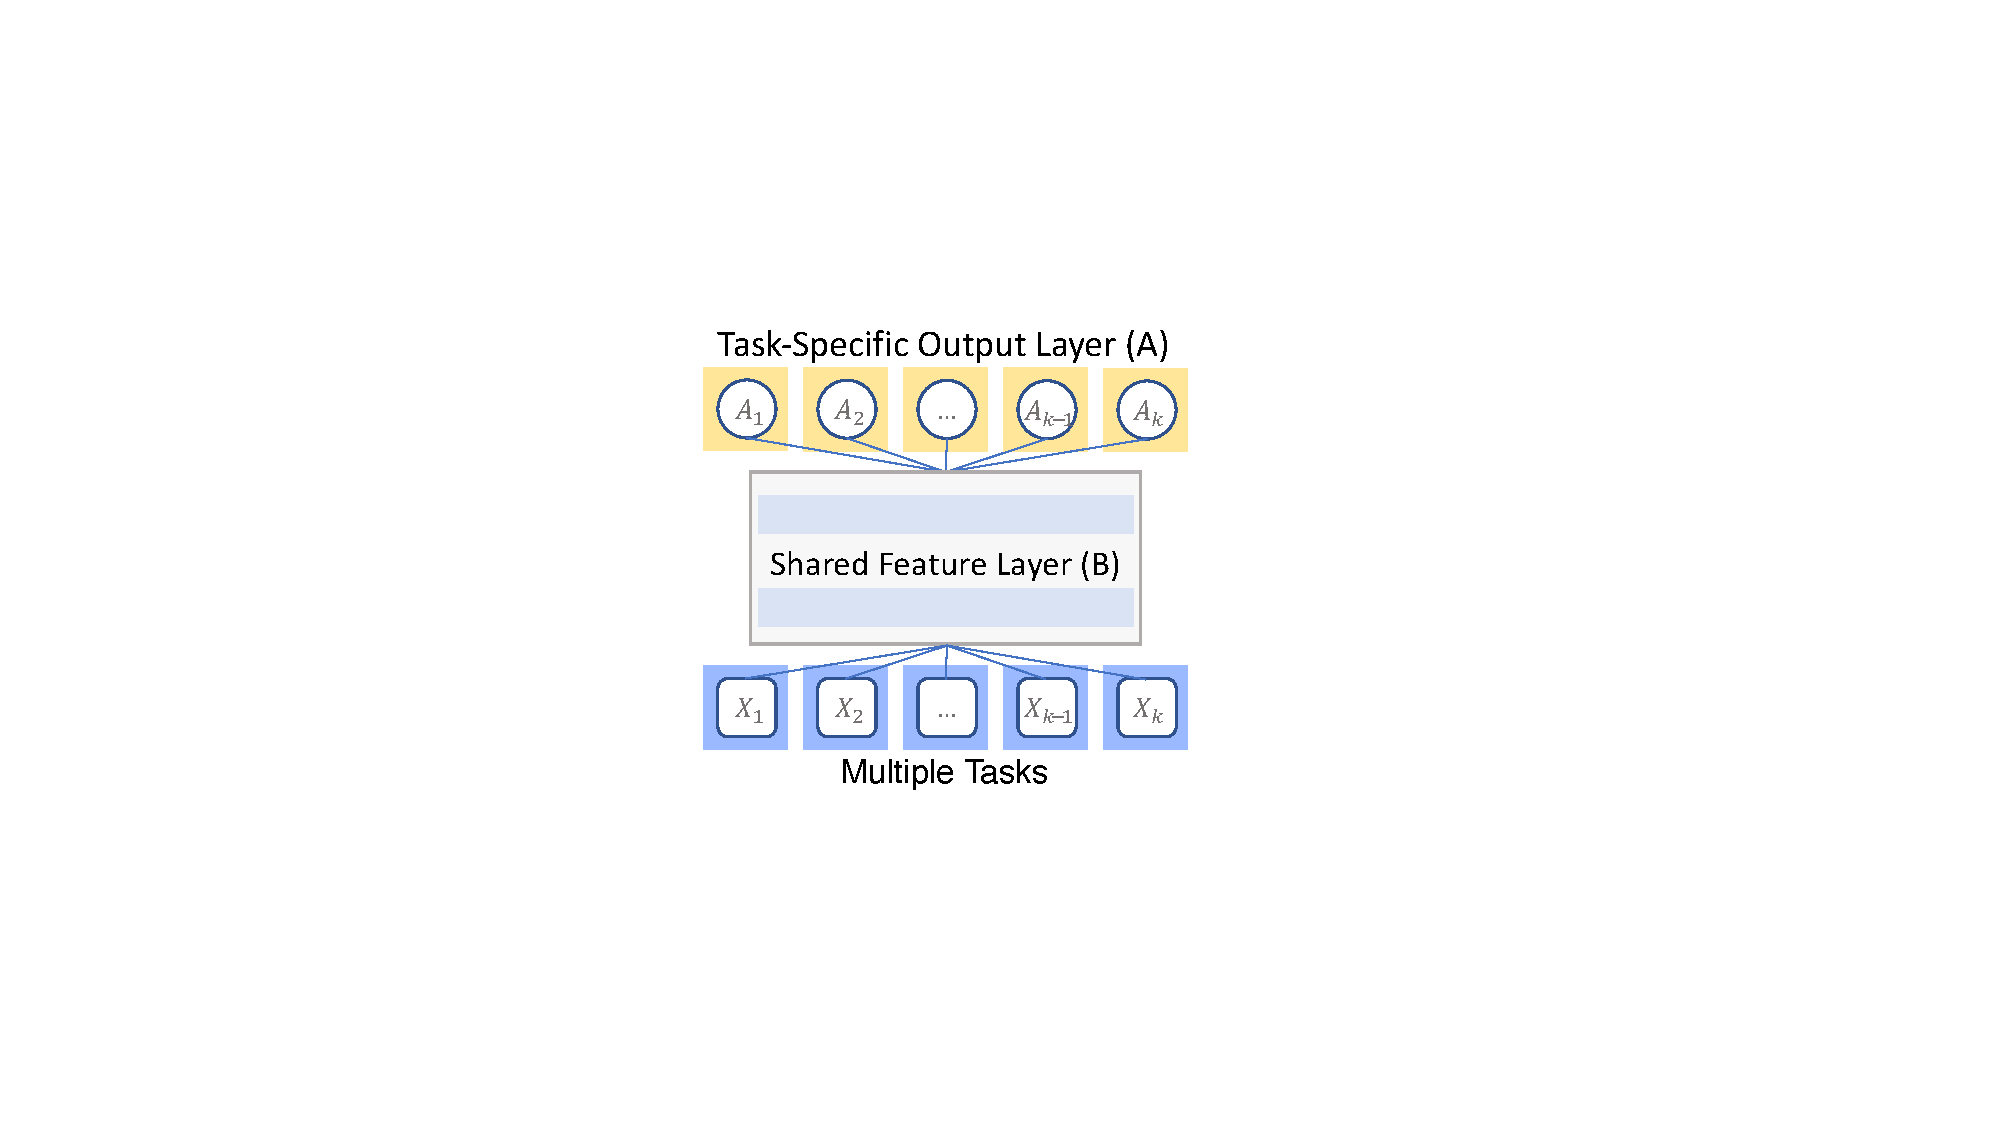
\includegraphics[width=0.45\textwidth,valign=t]{figures/mtl_model_arch.pdf}
		\caption{A hard parameter sharing architecture}
		\label{fig_intro_arch}
	\end{subfigure}\hfill
	\begin{subfigure}[t]{0.5\textwidth}
		\centering
		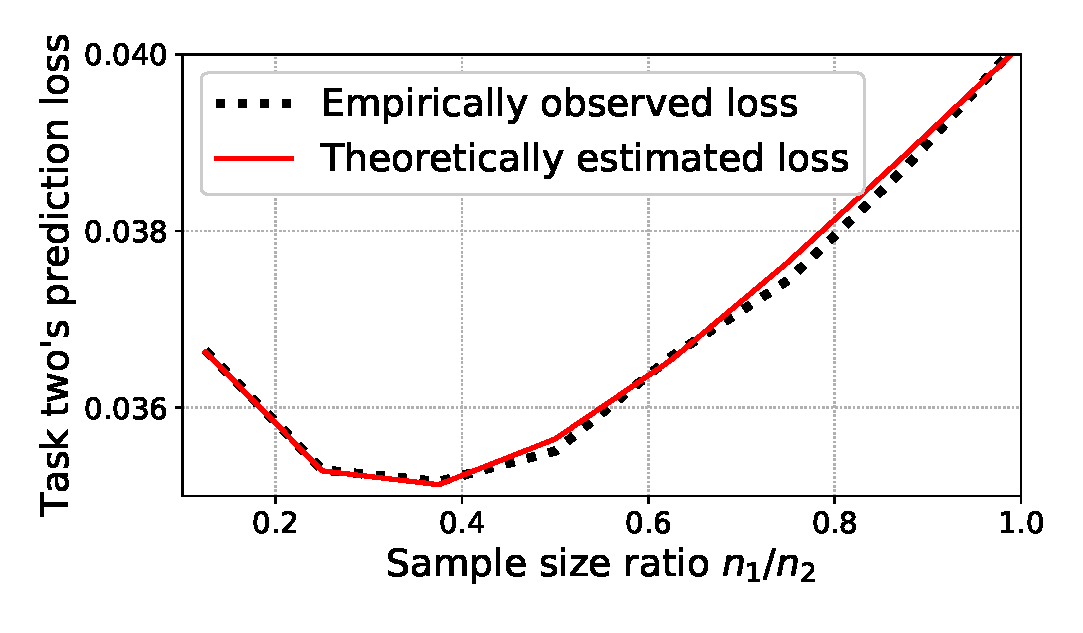
\includegraphics[width=0.745\textwidth,valign=t]{figures/sample_ratio_c2_400.eps}
		\caption{Varying sample size ratio}
		\label{fig_intro_sample_size_b}
	\end{subfigure}
	\vspace{-0.1in}
	\caption{
	Left: an illustrative picture of HPS.
	Right: an illustrative example of using HPS for two tasks $X_1, Y_1$ and $X_2, Y_2$ with sample size $n_1, n_2$, respectively.
	Increasing $n_1/n_2$ decreases task two's prediction loss initially but increase afterward. This phenomenon occurs due to different bias-variance tradeoffs as $n_1/n_2$ increases. Our result provides an estimated loss (solid line) that accurately matches the empirical loss (dotted line).
	See Section \ref{sec_simulation} for the precise setting.}
	\label{fig_intro_sample_size}
\end{figure*}



This paper presents new techniques to study hard parameter sharing and establishes a number of new results.
We consider regression analysis, which is arguably one of the most fundamental problems in statistics and machine learning.
We are interested in the \textit{high-dimensional} setting, where each dataset's sample size and feature dimension grow linearly instead of logarithmically.
This setting captures the fact that a single task's sample size is usually insufficient for accurate learning in many applications.
For example, if a dataset's sample size is only a constant factor of dimension in linear regression, the variance is also constant (cf. Fact \ref{fact_tr}).
The high-dimensional setting is challenging but is crucial for understanding how datasets' sample sizes impact generalization performance.

\subsection{Setup and Main Results}

%We assume that there are multiple datasets that all follow (potentially different) linear models.
%In each dataset, suppose the feature vector is $x = {\Sigma}^{1/2} z$, where $z \in \real^p$ has i.i.d entries with zero mean and unit variance, and the population covariance matrix $\Sigma \in\real^{p \times p}$ is deterministic and positive semidefinite.
Suppose we have $t$ datasets.
For each dataset $i$ from $1$ to $t$, let $n_i$ denote its sample size.
Let $X^{(i)} \in \real^{n_i \times p}$ denote dataset $i$'s feature covariates.
We assume that the label vector $Y^{(i)} \in \real^{n_i}$ for $X^{(i)}$ follows a linear model plus random noise.
We study the standard hard parameter sharing architecture:
a shared feature representation layer $B\in\real^{p\times r}$ for all datasets and a separate output layer $A_i \in \real^r$ for every dataset $i$.
See Figure \ref{fig_intro_arch} for an illustration.
%The width of $B$, denoted by $r$, plays an important role in regularization.
%As observed in Proposition 1 of \cite{WZR20}, if $r \ge t$, there is no regularization effect.
%Hence, we assume that $r < t$ in our study.
%For example, when there are only two tasks, $r = 1$ and $B$ reduces to a vector whereas $W_1, W_2$ become scalars.
We study the following minimization problem:
%	\item Separate each dataset $(X_i, Y_i)$ randomly into a training set $(X_i^{tr}, Y_i^{tr})$ and a validation set $(X_i^{val}, Y_i^{val})$.
%	The size of each set is described below.
%	\item Learn the shared layer $B$: minimize the training loss over $B$ and $W_1, \dots, W_t$, leading to a local minimum of $B$ that depends on $W_1, \dots, W_t$, denoted by $\hat{B} = \hat{B}(W_1, \dots, W_t)$.
%\vspace{-0.1in}
\begin{align}\label{eq_mtl}
			f(A, B) = \sum_{i=1}^t \norm{X^{(i)} B A_i - Y^{(i)}}^2,
\end{align}
%\vspace{-0.05in}
where $A = [A_1, A_2, \dots, A_t] \in \real^{r \times t}$.
Given a solution from minimizing $f(A, B)$, denoted by $(\hat{A}, \hat{B})$  (which we will specify below), let $\hat{\beta}_i^{\MTL} = \hat{B} \hat{A}_i$ denote the HPS estimator for task $i$.
The critical questions are:
(i) How well does the estimator work? In particular, how does the performance of the estimator scale with sample size?
(ii) For datasets with different sample sizes and covariate shifts, how do they affect the estimator?

\medskip
\noindent\textbf{Main results.}
Our first result (Theorem \ref{thm_many_tasks}) applies to multi-label prediction settings where all datasets have the same features (and sample size), and we want to make several predictions for every input (cf. examples in \cite{hsu2009multi}).
We analyze the global minimizer of $f(A, B)$, and provide a sharp bias-variance decomposition of its (out-of-sample) prediction loss for any task.
This setting is tractable even though in general, $f(A, B)$ is non-convex in $A$ and $B$ (e.g. matrix completion is a special case for suitably designed $X^{(i)}, Y^{(i)}$).
%We show that the prediction loss of HPS admits a clean bias-variance decomposition.
Our result implies that when all tasks have the same features but different labels, for any task, HPS helps reduce the task's variance compared to single-task learning but increases bias.

Our second result (Theorem \ref{thm_main_RMT}) applies to two tasks with arbitrarily different sample size ratios and covariate shifts.
While we can no longer characterize $f(A, B)$'s global minimum because of non-convexity, we can still provide a sharp bias-variance tradeoff of any local minimizer's prediction loss for both tasks.
Despite being a simple setting, we observe several non-trivial phenomena by varying sample size ratios and covariate shifts between the two tasks.
See Figure \ref{fig_intro_sample_size_b} for an illustration of the former.
Consequently, using our precise loss estimates, we observe several qualitative properties of HPS for varying dataset properties.
\begin{itemize}
	\item \textit{Sample efficiency (Example \ref{ex_same_cov})}:
	One advantage of combining multiple datasets is that the requirement for labeled data reduces compared to single-task learning, a phenomenon that \cite{ZSSGM18} has observed empirically.
	Our results further imply that HPS's sample efficiency depends on model-specific variances across tasks vs. the noise variance and is generally high when the latter is large.

	\item \textit{Sample size ratio (Example \ref{ex_sample_ratio})}: Increasing one task's sample size does not always reduce another task's loss. In a simplified setting, we find that the task loss either decreases first before increasing afterward or decreases monotonically depending on how fast the bias grows. These two trends result from different bias-variance tradeoffs. This result is surprising because previous generalization bounds in multi-task learning typically scale down as all tasks' sample sizes increase, thus do not apply for different sample size ratios.

	\item \textit{Covariate shift (Example \ref{ex_covshift})}: In addition to sample sizes, variance also scales with two datasets' covariate shifts. For a large sample size ratio, HPS's  variance is smallest when there is no covariate shift. Counterintuitively, for a small sample size ratio, having covariate shifts reduces variance through a complementary spectrum. We achieve this result through a novel characterization on the inverse of the sum of two sample covariance matrices with arbitrary covariate shifts. See our discussion of proof techniques below for details.
\end{itemize}

%First, we develop tight bounds for the bias and variance of the multi-task estimator for two tasks by applying recent development in random matrix theory \cite{erdos2017dynamical,isotropic,Anisotropic}.
%We observe that the variance of the multi-task estimator is \textit{always smaller} than single-task learning, because of added source task samples.
%On the other hand, the bias of the multi-task estimator is \textit{always larger} than single-task learning, because of model distances.
%Hence, the tradeoff between bias and variance determines whether the transfer is positive or negative.
%We provide a sharp analysis of the \textit{variance} that scales with sample size and covariate shift.
%We extend the analysis to the bias, which \textit{in addition} scales with {task similarity}.
%Combining both, we analyze the bias-variance tradeoff for two tasks in Theorem \ref{thm_main_informal} and extend the analysis to many tasks with the same features in Theorem \ref{thm_many_tasks}.
%For the setting of two tasks, we show how the variance of the multi-task estimator  scales with sample size and covariate shift in the following result.
%\textit{Our first contribution} is to develop a concentration bound that arises naturally from the bias-variance tradeoff of $\hat{\beta}_t^{\MTL}$ for two tasks.
%Let $\hat{\beta}_t^{\STL}$ denote the single-task estimator.
%Without loss of generality, let the $t$-th task denote the target task.
%Importantly, the target task's data size is a fixed constant times $p$ in the high-dimensional setting.
%Hence adding more labeled data can help improve its test performance.
%$B\in\real^{p\times r}$
%$\set{W_i \in \real^{r}}_{i=1}^t$

%Concretely, we show a tight bound on the trace of $(X_1^{\top}X_1 + X_2^{\top}X_2)^{-1}$, which
%Theorem \ref{lem_cov_shift_informal} allows us to analyze the bias-variance tradeoff of the multi-task estimator for two settings:
%(i) two tasks with arbitrary covariate shift; (ii) many tasks with no covariate shift.

%We shall assume that each task data follows a linear model, i.e. $y_i = X_i \beta_i + \varepsilon_i$, $1\le i\le k$.
%Here $\beta_i\in\real^p$ is the model parameter for the $i$-th task.
%Each row of $X_i\in\real^{n_i\times p}$ is assumed to be drawn i.i.d. from a fixed
%distribution with covariance matrix $\Sigma_i$.

%We extend our result to the transfer learning
%in the setting of high-dimensional linear regression.
%by pooling source task representations into the shared body of the hard parameter sharing architecture, following
%setting of Taskonomy by Zamir et al. \cite{ZSSGM18}.
%We prove that the bias of the transfer learning estimator is given by the projection of $\beta_t$ to the orthogonal subspace spanned by $\set{\beta_i}_{i=1}^{t-1}$.
%These results are described more precisely in Section \ref{sec_main}.

%Second, we explain the phenomena in Figure \ref{fig_model_shift_phasetrans} in isotropic and covariate shifted settings.
%We observe that negative transfer occurs as (a) \textit{task similarity}: tasks become more different; (b) \textit{data size}: source/target data size increases.
%\textbf{Task similarity:}
%\textbf{Data sizes:}
%\textbf{Covariate shift:}
%Furthermore, MTL performance is negatively affected when (c) \textit{covariate shift}: the covariance matrices of the two tasks become more different.
%\squishlist
%	\item We provide conditions to predict the effect of transfer as a parameter of model distance $\norm{\beta_1-\beta_2}$ (Section \ref{sec_similarity}).
%	As model distance increases, the bias becomes larger, resulting in negative transfer.
%	Our result predicts most of the empirical observations in Figure \ref{fig_model_shift} correctly.
%	It is crucial that the concentration result in Theorem \ref{lem_cov_shift_informal} is sufficiently precise so that we can explain the transition phenomena in Figure \ref{fig_model_shift} and \ref{fig_size}.
%	The unexplained observations are caused by an error term from the bias.
%	We discuss these in Section \ref{sec_insight}.
%	\item We provide conditions to predict transfer as a parameter of sample ratio $\rho_1/\rho_2$ (Section \ref{sec_data_size}).
%	Adding source task samples helps initially by reducing variance, but hurts eventually due to bias.
	%namely adding more labeled data from the source task does not always improve performance (Proposition \ref{prop_data_size}).
	%Theorem \ref{lem_cov_shift_informal} allows us to compare MTL performance under different covariate shifts.
%	\item For a special case of $\beta_1=\beta_2$, we show that MTL performs best when the singular values of $\Sigma_1^{1/2}\Sigma_2^{-1/2}$ are all equal  (Section \ref{sec_covshift}).
%	Otherwise, the variance reduces less with covariate shift.
%	Our theoretical bound matches the empirical curve in Figure \ref{fig_covariate}.
%\squishend
%In Section \ref{sec_insight}, we consider three components including task similarity, data size and covariate shift for a simplified isotropic setting of two tasks.
%We measure task similarity by how small is the distance between $\beta_1$ and $\beta_2$.
%Using our tool, we explain a transition from positive to negative transfer as task similarity decreases.
%		Furthermore, we show that negative transfer is more likely to occur when the source task labels are particularly noisy.
%		In Section \ref{sec_validate}, we validate the observation on text and image classification tasks.
%	In , we provide the trade-off between $\norm{\beta_1 - \beta_2}^2$ and a certain function $\Phi(\rho_1, \rho_2)$ to determine the type of transfer.
%We show that increasing the data size of the source task does not always improve performance for the target task in multi-task learning.
%Along the way, we analyze the benefit of MTL for reducing labeled data to achieve comparable performance to STL, which has been empirically observed in Taskonomy by Zamir et al. \cite{ZSSGM18}.
%We show that covariate shift, measured by $\Sigma_1^{1/2}\Sigma_2^{-1/2}$, is another cause for suboptimal performance for $\hat{\beta}_t^{\MTL}$.
%		We show that as $n_1 / n_2$ becomes large, having no covariate shift between the source and target tasks yields the optimal performance for the target task.
%		On the other hand, when $n_1 / n_2$ is small, there are counter examples where having the same covariance matrix is not necessarily the optimal choice.

%Our study also leads to several algorithmic consequences with practical interest.
%First, we show that single-task learning results can help to predict positive or negative transfer for multi-task learning.
%We validate this observation on ChestX-ray14 \cite{chexnet17} and sentiment analysis datasets \cite{LZWDA18}.

%Third, we provide a fine-grained insight on a covariance alignment procedure proposed in \cite{WZR20}.
%We show that the alignment procedure provides more significant improvement when the source/target sample ratio is large.
%Finally, we validate our three theoretical findings on sentiment analysis tasks.

% plus an identity matrix,  due to lack of freeness
%\HZ{add why this is challenging}

Finally, we discuss the practical implications of our work.
Our sample size ratio study implies a concrete progressive training procedure that gradually adds more data until performance drops.
For example, in the setting of Figure \ref{fig_intro_sample_size_b}, this procedure will stop right at the minimum of the local basin.
We conduct further studies of this procedure on six text classification datasets and observe that it reduces the computational cost by $65\%$ compared to a standard round-robin training procedure while keeping the average accuracy of all tasks simultaneously.

\medskip
\noindent\textbf{Proof techniques.}
There are two main ideas in our analysis. The proof of our first result uses a geometric intuition that hard parameter sharing finds a ``rank-$r$'' approximation of the datasets.
We carefully keep track of the concentration error between the global minimizer of $f(A, B)$ and its population version (cf. equation \eqref{eq_A_star}).
The proof of our second result is significantly more involved because of different sample sizes and covariate shifts. We show that the inverse of the sum of two sample covariance matrices with arbitrary covariate shifts converges to a deterministic diagonal matrix asymptotically (cf. Theorem \ref{thm_main_RMT}).
We use recently developed techniques from random matrix theory to show a sharp convergence rate.
% to obtain a sharp estimate on the..., which is commonly referred to as the \emph{local law}.
%\HZ{add several sentences on the technical insight}
One limitation of our analysis is that in Example \ref{ex_sample_ratio}, there is an error term that can result in vacuous bounds for very small $n_1$ (cf. equation \eqref{cor_MTL_error}).
We believe our result has provided significant initial insights, and it is an interesting question to tighten our result.
See Section \ref{sec_conclude} for more discussions of the technical challenge.

%This part introduces a positive variance reduction effect from adding the source labels.
%Hence, whether $\te(\hat{\beta}_t^{\MTL}) < \te(\hat{\beta}_t^{\STL})$ is determined precisely by the tradeoff between the negative effect of the bias term and the positive effect of the variance term!
%(i) the negative effect from model shift bias.
%(ii) the positive effect from variance reduction;


\subsection{Related Work}

There is a large body of classical and recent works on multi-task learning.
We focus our discussion on theoretical results and refer interested readers to several excellent surveys for general references \cite{PY09,ZY17,V20}.
The early work of \cite{B00,BS03,M06} studied multi-task learning from a theoretical perspective, often using uniform convergence or Rademacher complexity based techniques.
An influential paper by \cite{BBCK10} provides uniform convergence bounds that combine multiple datasets in certain settings.
One limitation of uniform convergence based techniques is that the results often assume that all  tasks have the same sample size, see e.g. \cite{B00,MPR16}.
Moreover, these techniques do not apply to the high-dimensional setting because the results usually require a sample size of at least $p \log p$.

Our proof techniques use the so-called local law of random matrices \cite{erdos2017dynamical}, a recent development in the random matrix theory literature.
In the single-task case, \cite{isotropic} first proved such a local law for sample covariance matrices with isotropic covariance.
\cite{Anisotropic} later extended this result to arbitrary covariance matrices.
%On the other hand, one may derive the asymptotic result in Theorem \ref{thm_main_RMT} with error $\oo(1)$ using the free addition of two independent random matrices in  theory .
These techniques provide almost sharp convergence rates to the asymptotic limit compared to other methods such as free probability \cite{nica2006lectures}.
To the best of our knowledge, we are not aware of any previous results in the multi-task case, even for two tasks (with arbitrary covariate shifts).

The problem we study here is also related to high-dimensional prediction in transfer learning \cite{li2020transfer,bastani2020predicting} and distributed learning \cite{dobriban2018high}.
For example, \cite{li2020transfer} provide minimax-optimal rates to predict a target regression task given multiple sparse regression tasks.
One closely related work is \cite{WZR20}, which studied hard parameter sharing for two linear regression tasks.
However, their results only apply to sample size regimes at least logarithmic factors of dimension.
%\cite{WZR20} (and an earlier work by \cite{KD12}) observed that the shared layer size $r$ in hard parameter sharing plays a critical role of regularization.
%Linear models in multi-task learning have been studied in various settings, including online learning \cite{CCG10,DCSP18}, sparse regression \cite{LPTV09,LPVT11}, and representation learning \cite{BHKL19}.

%Our setting is closely related to domain adaptation \cite{DM06,BB07,BC08,DH09,MMR09,CWB11,ZS13,NB17,ZD19}.
%The important distinction is that we focus on predicting the target task using a hard parameter sharing model.
%For such models, their output dimension plays an important role of regularization \cite{KD12}.
%Below, we describe several lines of work that are most related to this work.

%Some of the earliest works on multi-task learning are Baxter , Ben-David and Schuller \cite{BS03}.
%Mauer \cite{M06} studies generalization bounds for linear separation settings of MTL.
%The benefit of learning multi-task representations has been studied for learning certain half-spaces \cite{MPR16} and sparse regression \cite{LPTV09,LPVT11}.
%Our work is closely related to Wu et al. \cite{WZR20}.
%While Wu et al. provide generalization bounds to show that adding more labeled helps learn the target task more accurately, their techniques cannot be used to explain when MTL outperforms STL.
%\todo{spell out the challenge more explicitly}

%Ando and Zhang \cite{AZ05} introduces an alternating minimization framework for learning multiple tasks.
%Argyriou et al. \cite{AEP08} present a convex algorithm which learns common sparse representations across a pool of related tasks.
%Evgeniou et al. \cite{EMP05} develop a framework for multi-task learning in the context of kernel methods.
%\cite{KD12} observed that controlling the capacity can outperform the implicit capacity control of adding regularization over $B$.
%The multi-task learning model that we have focused on uses the idea of hard parameter sharing \cite{C93,KD12,R17}.
%We believe that our theoretical framework can apply to other approaches to multi-task learning.



\smallskip
\noindent\textbf{Organizations.}
The rest of this paper is organized as follows.
In Section \ref{sec_same}, we present the bias-variance decomposition for hard parameter sharing.
In Section \ref{sec_diff}, we describe how varying sample sizes and covariate shifts impact hard parameter sharing using random matrix theory.
In Sections \ref{sec_simulation}, we validate our results in simulations.
In Section \ref{sec_conclude}, we summarize our work and discuss future work.
Section \ref{sec_text} describes our study on text classification tasks.
Section \ref{app_proof_error_same_cov}, \ref{appendix RMT}, and \ref{app_iso_cov} present proofs of our results.

\medskip
\noindent\textbf{Notations.}
%Let $\cE \define [\varepsilon_1, \varepsilon_2, \dots, \varepsilon_t] \in \real^{n \times t}$ denote the random noise.
%We can also write $Y = XB^{\star} + \cE$.
%Let $A = [A_1, A_2, \dots, A_t] \in \real^{r\times t}$ be a matrix notation that contains all the output layer parameters.
For an $n\times p$ matrix $X$, let $\lambda_{\min}(X)$ denote its smallest singular value and $\norm{X}$ denote its largest singular value.
Let $\lambda_1(X), \lambda_2(X), \cdots, \lambda_{p\wedge n}(X)$ denote the singular values of $X$ in decreasing order.
Let $X^+$ denote the Moore-Penrose psuedoinverse of $X$.
We refer to random matrices of the form $\frac {X^\top X} n$ as sample covariance matrices.
We say that an event $\Xi$ holds with high probability if the probability that $\Xi$ happens goes to $1$ as $p$ goes to infinity.
We use the big-O notation $g(n) = \OO(f(n))$ if there exists a constant $C$ such that $g(n) \le C \dot f(n)$ for large enough $n$. Moreover, we use the notation $g(n)\lesssim f(n)$ if $g(n) = \OO(f(n))$, and the notation $g(n)\sim f(n)$ if $g(n) \lesssim f(n))$ and $f(n) \lesssim g(n)$. In this paper, we will often write an identity matrix $\id_{n\times n}$ as $1$ without causing any confusions. 
%We shall use $\oo(1)$ to mean a small positive quantity that converges to 0 as $p$ goes to infinity.

\section{Transfer learning for high-dimensional linear regression}\label{sec_HPS}
In this section, we define our model for the setting of transfer learning, and introduce several transfer learning estimators that will be considered in this paper. 

\subsection{The model}
Consider the transfer learning setting with two data sets. We denote their sample sizes by $n_1$ and $n_2$. For $i=1,2,$ Let $X^{(i)} \in \real^{n_i \times p}$ denote dataset $i$'s feature covariates. We assume that the label vector $Y^{(i)} \in \real^{n_i}$ for $X^{(i)}$ follows a linear model plus random noise:
$$Y^{(i)}= X^{(i)}\beta^{(i)} + \varepsilon^{(i)},\quad i=1,2.$$
In this paper, we make the following assumptions on feature covariates $X^{(i)}$ and the noise vectors $\varepsilon^{(i)}$. We remark that all these assumptions are natural in high-dimensional statistics. 

We assume that the row vectors of $X^{(i)}$ are i.i.d. centered random vectors with  population covariance matrix $\Sigma^{(i)}$. More precisely, let 
\be\label{XofZ}X^{(i)} = Z^{(i)} (\Sigma^{(i)})^{1/2} \in \real^{n_i\times p},\quad i=1,2, \ee
where each $\Sigma^{(1)}$ and $\Sigma^{(2)}$ are $p\times p$ deterministic positive definite symmetric matrices, and $Z^{(1)}=(z^{(1)}_{ij})$ and $Z^{(2)}=(z^{(2)}_{ij})$ are $n_1\times p$ and $n_2\times p$ random matrices with real i.i.d. entries satisfying
\begin{equation}\label{assm1}
\mathbb{E} z^{(1)}_{ij}=\mathbb{E} z^{(2)}_{ij} =0, \ \quad \ \mathbb{E} \vert z^{(1)}_{ij} \vert^2=\mathbb{E} \vert z^{(2)}_{ij} \vert^2 =1, 
\end{equation}
Furthermore, we assume that the entries $z^{(1)}_{ij}$ and $z^{(2)}_{ij}$ have finite $\varphi$-th moment for some constant $\varphi>4$:
\be \label{conditionA2}
\mathbb{E} \vert z^{(1)}_{ij} \vert^\varphi  \le \tau^{-1},\quad \mathbb{E} \vert  z^{(2)}_{ij} \vert^\varphi   \le \tau^{-1}
\ee
for a small constant $\tau>0$. We assume that $\Sig^{(i)}$ has eigendecomposition
\be\label{eigen}
\Sig^{(i)}= O_i\Lambda_i O_i^\top, \quad  \Lambda_1=\text{diag}(\si_1^{(i)}, \ldots, \si^{(i)}_n),  \quad i=1,2,
\ee
where $O_i$ is the eigenmatrix and the eigenvalues satisfy that
\begin{equation}\label{assm3}
 \tau \le  \si^{(i)}_p \le\cdots\le \si^{(i)}_2 \le \si^{(i)}_1 \le \tau^{-1} \quad i=1,2.
\ee
%for a small constant $\tau>0$. 

We assume that $\varepsilon^{(1)} \in \real^{n}$ and $\varepsilon^{(2)} \in \real^{n}$ are two independent random noise vectors with i.i.d entries of mean zero, variance $\sigma^2$, and bounded moment up to any order: for any fixed $k\in \N$, there exists a constant $C_k>0$ such that 
\be\label{eq_highmoments}
\E  | \ve^{(1)}_{i} |^k \le C_k,\quad \E  | \ve^{(2)}_{i} |^k \le C_k.
\ee
Finally, we assume that $\beta^{(1)}$ and $\beta^{(2)}$ are two arbitrary deterministic or random vectors that are independent of $X^{(1)}$, $X^{(2)}$, $\varepsilon^{(1)}$ and $\varepsilon^{(2)}$. 
%Moreover, we assume that 
%\be\label{eq_SNR}
%\tau\le \frac{\|\beta^{(1)}\|^2}{\|\beta^{(2)}\|^2} \le \tau^{-1},\quad  \frac{\|\beta^{(1)}\|^2}{\sigma^2} \ge \tau,
%\ee
%for a small constant $\tau >0$. The first condition means that the norms of the two model parameters $\beta^{(1)}$ and $\beta^{(2)}$ are comparable, while the second condition means that the singal-to-noise ratio cannot be too small.
 
In this paper, we consider the high-dimensional setting, where the sample ratios satisfy that  %We assume that the aspect ratios $d_1:= p/n_1$ and $d_2:=p/n_2$ satisfy that 
\be\label{assm2}
1+\tau \le \rho_1:=\frac{n_1}{p} \le p^{\tau^{-1}}, \quad 1+\tau \le \rho_2:=\frac{n_2}{p} \le p^{\tau^{-1}}, \quad \tau \le \frac{\rho_1}{\rho_2}\le \tau^{-1},
\ee
for a small constant $\tau >0$. If $\rho_i>p^{\tau^{-1}}$, $i=1,2$, we are basically in the low-dimensional region, where the law of large numbers and central limit theorem already  give good enough results without using the theory developed in this paper. The lower bounds $\rho_1> 1+\tau$ and ${\rho_2 > 1+ \tau}$ 
are to ensure that the sample covariance matrices $  (X^{(1)})^\top X^{(1)} $ and $  (X^{(2)})^\top X^{(2)} $ are non-singular with high probability, so that the ordinary least squares (OLS) estimator is well-defined for the linear regression problem on each task.  


We summarize our basic assumptions here for future reference.
\begin{assumption}\label{assm_big1}
Let $\tau$ be a small constant. 
\begin{enumerate}
\item  $X^{(1)}$ and $X^{(2)}$ take the form \eqref{XofZ}, where $Z^{(1)}$ and $Z^{(2)}$ are respectively $n_1\times p$ and $n_2\times p$ random matrices with i.i.d. entries satisfying (\ref{assm1}) and \eqref{conditionA2}, $\Sig^{(1)}$ and $\Sig^{(2)}$ are deterministic positive definite symmetric matrices satisfying \eqref{eigen} and \eqref{assm3}. %and (\ref{assm2}). We assume that $T$ is an $M\times M$ deterministic diagonal matrix satisfying (\ref{simple_assumption}) and (\ref{assm3}).  
 
\item $\varepsilon^{(1)} \in \real^{n}$ and $\varepsilon^{(2)} \in \real^{n}$ are random vectors independent from $X^{(1)}$ and $X^{(2)}$, and with i.i.d entries of mean zero, variance $\sigma^2$, and bounded moments as in \eqref{eq_highmoments}.  

\item $\beta^{(1)}$ and $\beta^{(2)} $ are independent of $X^{(1)}$, $X^{(2)}$, $\varepsilon^{(1)}$ and $\varepsilon^{(2)} $. %, and satisfy \eqref{eq_SNR}. 
 
\item $\rho_{1}$ and $\rho_{2}$ satisfy \eqref{assm2}.

\end{enumerate}
\end{assumption}
 
\subsection{Transfer learning estimators}

\FY{Introduce some popular transfer learning estimators: total loss estimator, and model averaging estimator.}

We study the standard hard parameter sharing architecture: a shared feature representation layer $B\in\real^{p}$ for all datasets and a separate output layer $A_i \in \real$ for every dataset $i$. Then we study the following minimization problem:
\begin{align}\label{eq_tsl}
			f(A, B) = \norm{X^{(1)} B A_1 - Y^{(1)}}^2 + \norm{X^{(2)} B A_2 - Y^{(2)}}^2,
\end{align}
where we abbreviate $A = [A_1, A_2]$. Let $(\hat{A}, \hat{B})$ be the minimizer of $f(A, B)$. We define the hard parameter sharing (HPS) estimator for task $i$ as 
\be\label{def_HPS}\hat{\beta}_i^{\MTL} = \hat{B} \hat{A}_i,\quad i=1,2.\ee


For the optimization objective $f(A, B)$ in \eqref{eq_tsl}, using the local optimality condition $\frac{\partial f}{\partial B} = 0$, we can solve that  
	\begin{align}
		\hat{B} = A_2^{-1} \hat \Sigma(a)^{-1} \left[a (X^{(1))})^{\top}Y^{(1)} +  (X^{(2)})^{\top}Y^{(2)}\right], \label{eq_Bhat_2task} %\\
		%&= (B^\star A ^{\top}) (A A^{\top})^{-1} + (X^{\top}X)^{-1}X^{\top}   \bigbrace{\sum_{j=1}^t \varepsilon_i A_i^{\top}} (A  A^{\top})^{-1}.
	\end{align}
where we denote $a:=A_1/A_2$ and $\hat \Sigma(a):= a^2 (X^{(1)})^\top X^{(1)}  + (X^{(2)})^\top X^{(2)}$.
Applying $\hat B$ to equation \eqref{eq_tsl}, we obtain an objective that only depends on $a $ as follows %\HZ{$A$ has been used to denote the output layers. Could you replace $A$ with another symbol (say $x$)?}
 \begin{align}
		 g(a) \define & \left\| X^{(1)} \hat\Sigma(a)^{-1} (X^{(2)})^\top X^{(2)} (a\beta^{(2)}-\beta^{(1)}) \right. \nonumber\\
			& \left. + \left(a^2 X^{(1)}\hat \Sigma(a)^{-1} (X^{(1)})^\top-\id_{n_1\times n_1}\right)\epsilon^{(1)}+ a X^{(1)}\hat \Sigma(a)^{-1} (X^{(2)})^\top \epsilon^{(2)} \right\|^2 \nonumber\\
		   +& \left\| X^{(2)} \hat \Sigma(a)^{-1} (X^{(1)})^\top X^{(1)} (a\beta^{(1)}-a^2\beta^{(2)}) \right. \nonumber\\
		  &\left.+ \left(X^{(2)}\hat\Sigma(a)^{-1} (X^{(2)})^\top-\id_{n_2\times n_2}\right)\epsilon^{(2)} + a X^{(2)}\hat \Sigma(a)^{-1} (X^{(1)})^\top \epsilon^{(1)} \right\|^2. \label{eq_mtl_A12}
	\end{align}
Let $\hat a$ be the minimizer of $g(a)$. Throughout this paper, we regard $Y^{(1)}$ as the source data, and $Y^{(2)}$ as the target data.  Then the HPS estimator \eqref{def_HPS} for the target task 2 is
\be\label{HPS_est}
\hat{\beta}_2^{\MTL} (\hat a) = \hat \Sigma(\hat a)^{-1}  \left[\hat a (X^{(1))})^{\top}Y^{(1)} +  (X^{(2)})^{\top}Y^{(2)}\right].
\ee

In this paper, we study the out-of-sample predication loss (test error) of $\hat{\beta}_2^{\MTL} (\hat a)$. Consider a test data point $(x,y)$ generated from the same model as task 2: $y= x^\top \beta^{(2)} + \ve$, where $x \in \R^p$ and $\ve\in \R$ are independent of $X^{(1)}$, $X^{(2)}$, $\varepsilon^{(1)}$ and $\varepsilon^{(2)}$, and only $x$ is observable. We want to use $x^\top \hat{\beta}_2^{\MTL} (\hat a) $ to predict $y$, and we measure the predication loss using the mean squared error
$$\exarg{x}{\left\|y-x^\top \hat{\beta}_2^{\MTL} (\hat a) \right\|^2}= \left\|(\Sigma^{(2)})^{1/2} \left(\hat{\beta}_2^{\MTL} (\hat a)  - \beta^{(2)}\right)\right\|^2 + \sigma^2.  $$ 
Since $\sigma^2$ is a constant that does not depend on the model, we ignore it and define the predication loss as
\be\label{HPS_loss}
L(\hat{\beta}_2^{\MTL}(\hat a)):= \left\|(\Sigma^{(2)})^{1/2} \left(\hat{\beta}_2^{\MTL} (\hat a)  - \beta^{(2)}\right)\right\|^2 .
 \ee
We will compare it to the out-of-sample predication loss $L(\hat{\beta}_2^{\STL})$ of the single-task OLS estimator 
$$\hat \beta^{\STL}= [(X^{(2)})^\top X^{(2)}]^{-1}(X^{(2)})^\top Y^{(2)}$$ as a baseline.  

Plugging \eqref{HPS_est} into \eqref{HPS_loss}, we get
\begin{align}
L(\hat{\beta}_2^{\MTL}(\hat a))  =  &\left\| (\Sigma^{(2)})^{1/2}\hat \Sigma(\hat a)^{-1} (X^{(1)})^\top X^{(1)} (\hat a\beta^{(1)}-\hat a^2\beta^{(2)}) \right. \nonumber\\
&\left. +(\Sigma^{(2)})^{1/2}\hat \Sigma(\hat a)^{-1} \left[ (X^{(2)})^\top \epsilon^{(2)} + \hat a  (X^{(1)})^\top \epsilon^{(1)} \right]\right\|^2.\label{Lbeta_HPS}
\end{align}
Note that if we replace $\hat a$ with a fixed number $a$ in \eqref{Lbeta_HPS}, then taking the expectation over $\ve^{(1)}$ and $\ve^{(2)}$, we can get a clean bias-variance decomposition of the predication loss:
\be\label{partial-L} \exarg{\ve^{(1)},\ve^{(2)}}{L(\hat{\beta}_2^{\MTL}(a)) } = L_{\bias} (a) + L_{\var}(a),\ee
where 
\be\label{Lbias} L_{\bias} (a) := \left\| (\Sigma^{(2)})^{1/2}\hat \Sigma(a)^{-1} (X^{(1)})^\top X^{(1)} \left(a\beta^{(1)}- a^2\beta^{(2)}\right) \right\|^2 \ee
is called the bias term, which depends on the model bias between task 1 and task 2, and
\be\label{Lvar}  L_{\var}(a):=\sigma^2  \bigtr{{\Sigma^{(2)}\hat \Sigma(a)^{-1}  }} \ee
is called the variance term, which depends on the noise variance. Using concentration of the noise vectors $\ve^{(1)}$ and $\ve^{(2)}$, we can show that $L(\hat{\beta}_2^{\MTL}(a))$ is close to \eqref{partial-L} up to a small error as in the next lemma. In this paper, we say that an event $\Xi$ holds \emph{with high probability} (w.h.p.) if $\mathbb P(\Xi)\to 1$ as $p\to \infty$.
%predication loss for the HPS and OLS estimators. 

 
 \begin{lemma}\label{lem_HPS_loss}
 Under Assumption \ref{assm_big1}, for any small constant $\e>0$ and large constant $C>0$, there exists a high probability event $\Xi$, on which the following estimates hold uniformly in $a\in \R$: 
\begin{align}
L(\hat{\beta}_2^{\MTL}(a)) &=\left[ 1+ \OO(p^{-1/2+c})\right]\cdot \left[L_{\bias} (a) + L_{\var}(a)\right] \nonumber\\
&+ \OO \left[ p^{-C}\left( \|\beta^{(1)} \|^2  +  \|\beta^{(2)} \|^2\right)   \right], \label{L_HPS_simple}
\end{align}
and 
\begin{align}
L(\hat{\beta}_2^{\STL} ) &= \left[ 1+ \OO(p^{-1/2+c})\right] \cdot \sigma^2  \bigtr{\Sigma^{(2)} [(X^{(2)})^\top X^{(2)}]^{-1}  }  . \label{L_STL_simple}
\end{align}
%Moreover, there exists a constant $C_0>0$ such that with high probability,
%\be\label{loss_large}
%g(a) > g(0) \quad \text{for all $a$ such that }|a|\ge C_0.
%\ee
%with high probability for any small constant $\e>0$. 
\end{lemma}

Since \eqref{L_HPS_simple} holds uniformly for all $a\in \R$, we can also apply it to $\hat{\beta}_2^{\MTL}(\hat a)$, where $\hat a$ is a random variable that may depend on $\ve^{(1)}$ and $\ve^{(2)}$. In practice, the parameter $ a$  is up to one's choice and may not be the global minimizer, so we have stated the result for an completely arbitrary $a$. (In fact, the optimization objective $g(a)$ is generally non-convex, so in some cases one can only find a local minimizer.) For a fixed $a\in \R$, the proof of \eqref{L_HPS_simple} is based on the sharp concentration bounds in Lemma \ref{largedeviation} of the supplement \cite{MTL_suppl}. To extend uniformly to all $a\in \R$, we will use a standard $\ve$-net argument, which leads to a small error $ p^{-C}\left( \|\beta^{(1)} \|^2  +  \|\beta^{(2)} \|^2\right) $. Note that this error is negligible unless $\beta^{(1)}$ and $ a\beta^{(2)}$ cancel each other almost exactly, and the noise variance $\sigma$ is very small. The proof of Lemma \ref{lem_HPS_loss} will be given in Appendix  \ref{app_firstpf} of the supplement \cite{MTL_suppl}. 

%In this section, we show that the prediction loss of hard parameter sharing admits a clean bias-variance decomposition, when all tasks have the same features.




For the single-task predication loss \eqref{L_STL_simple}, we can calculate its asymptotic limit exactly using the following classical result in multivariate statistics.
 
\begin{lemma}[Theorem 2.4 of \cite{isotropic} and Theorem 3.14 of \cite{DY}]\label{fact_tr}
	%Let $X  \in \real^{n\times p}$ be a random matrix that satisfies Assumption \ref{assume_rm}.
	%Let $\Sigma\in\real^{p\times p}$ denote the population covariance matrix of $X$.
	Under Assumption \ref{assm_big1}, we have that
		\[ \bigtr{\Sigma^{(2)} \frac1{(X^{(2)})^\top X^{(2)} }  } = \bigtr{ \frac1{(Z^{(2)})^\top Z^{(2)} }  } = \frac{p}{n_2 - p} \cdot \left[1+ \OO\left( \frac{p^{\e}}{\sqrt{np}} \right)\right] \]
		with high probability for any small constant $\e>0$.
\end{lemma}
 %The above result has a long history in random matrix theory.
If the entries of $Z^{(2)}$ are i.i.d. Gaussian, then this result follows from the classical result for the mean of inverse Wishart distribution \cite{anderson1958introduction}. For a general non-Gaussian $Z^{(2)}$, this result can be obtained using the well-known Stieltjes transform method (cf. Lemma 3.11 of \cite{bai2009spectral}). Here we have presented the results from \cite{isotropic,DY}, which give an almost sharp convergence rate. With Lemma \ref{fact_tr}, we obtain that w.h.p.,
\begin{align}
L(\hat{\beta}_2^{\STL} ) &= \left[ 1+ \OO(p^{-1/2+c})\right] \cdot \frac{p \sigma^2 }{n_2-p}   . \label{L_STL_simple01}
\end{align}
 

On the other hand, much less is known about the predication loss of the HPS estimator. In particular, its exact dependence on the model parameters, including the model bias, noise variance, sample sizes, and population covariance matrices, is not well-understood so far. \FY{What is known so far about this topic?} In the rest of this paper, we give a rigorous analysis of the bias term \eqref{Lbias} and variance term \eqref{Lvar} in three different settings of increasing complexity: (i) same covariates $X^{(1)}=X^{(2)}$; (ii) independent $X^{(1)}$ and $X^{(2)}$ with different sample sizes and same population covariance matrices $\Sigma^{(1)}=\Sigma^{(2)}$; (iii) independent $X^{(1)}$ and $X^{(2)}$ with different sample sizes and different population covariance matrices. In each case, we provide the exact asymptotic bias and variance limits, together with almost sharp convergence rates.  
In particular, we will use our results to analyze the effect of the following factors: \emph{bias-variance tradeoff}, \emph{sample sizes}, and \emph{covariate shift}.  

{\cor discuss about the bias-variance trade-off}
%However, to the best of our knowledge, the asymptotic limit of $L(\hat{\beta}_2^{\MTL}(a))$ has never been calculated exactly in any high-dimensional setting. 

 
\section{Predication loss for HPS estimator}
	
\subsection{Varying sample sizes} \label{sec_sizeratio}

 In this section, we consider the setting where $X^{(1)}$ and $X^{(2)}$ are independent and have the same population covariance matrices $\Sigma^{(1)}=\Sigma^{(2)}$. However, the two tasks can have different sample sizes $n_1\ne n_2$. In this case, we can obtain the exact asymptotic limits of the bias term \eqref{Lbias} and the variance term \eqref{Lvar}. We will use these results to illustrate the effect of the sample sizes on the predication loss of the $\MTL$ estimator.

\begin{theorem}\label{cor_MTL_loss}
Under Assumption \ref{assm_big1} holds, suppose that $\Sigma^{(1)}=\Sigma^{(2)}$ and the entries of $Z^{(1)}$ and $Z^{(2)}$ are i.i.d. Gaussian random variables. Then for any small constant $\e>0$ and large constant $C>0$, there exists a high probability event $\Xi$, on which the following estimates hold uniformly in all $a\in \R$: 
\be\label{Lvar_samplesize}
L_{\var}(a)= \left[ \cal L_1(a)+ \OO\left(\frac{p^{c}}{n_1}\right)\right] \cdot   \sigma^2 ,
\ee
and 
\begin{align}
L_{\bias}(a)&= \left[ \cal L_2(a)+  \OO\left(p^{-1/2+c}\right)\right]   \|\beta^{(1)}-a\beta^{(2)}\|^2 \nonumber\\
&+ \OO \left[ p^{-C}\left( \|\beta^{(1)} \|^2  +  \|\beta^{(2)} \|^2\right)   \right].\label{Lbias_samplesize}
	%-\left[1- \left( 1-\frac{1}{\sqrt{\rho_1}}\right)^4\right] pd^2\cdot \frac{\rho_1^2 (\rho_1+\rho_2)}{(\rho_1 + \rho_2 - 1)^3} +\OO(p^{-c}\sigma^2)  \le
	%   \left|L(\hat{\beta}_2^{\MTL}) - \frac{2d^2 n_1^2 (n_1 + n_2)}{(n_1 + n_2 - p)^3} -\frac{\sigma^2 p}{n_1 + n_2 - p}  \right|
	% \le \varepsilon \cdot \frac{2d^2 n_1^2 (n_1 + n_2)}{(n_1 + n_2 - p)^3} +  \OO(p^{-c/2}).\label{cor_MTL_error}
	%\left[\left( 1+\frac{1}{\sqrt{\rho_1}}\right)^4-1\right] d^2\cdot \frac{\rho_1^2 (\rho_1+\rho_2)}{(\rho_1 + \rho_2 - 1)^3} \\
	%& +C \left[(p^{-c_\varphi}+p^{-c_\infty/2})(\sigma^2 +d^2)+p^{-c_\infty}\kappa^2 + %\frac{d^4+\sigma^2 d^2}{\kappa^2}\right],\nonumber
	 \end{align}
Here we define the functions  
\begin{align*}
&\cal L_1(a):= \frac{2p}{  {n_2} (1-\xi_2) + a^2 n_1 (1-\xi_1)+ \sqrt{[ {n_2} (1-\xi_2) +a^2 n_1 (1-\xi_1)]^2 + 4a^2{n_2}{n_1} (\xi_1+\xi_2 -\xi_1\xi_2)}}, \\
&\cal L_2(a): = \frac1{a^2}\cdot \frac{1- 2\frac{\cal L_1(a)}{\xi_2[1 + \cal L_1(a)]} + \kappa(a)}{1- \xi_2 \kappa(a)},
\end{align*}
where we abbreviate $\xi_1:=p/n_1$, $\xi_2:=p/n_2$ and
\begin{align*}
\kappa(a):= \frac{\cal L_1(a)^2}{\xi_2^2[1+\cal L_1(a)]^2}  \left[1 - \frac{a^4 \cal L_1(a)^2 }{\xi_1[1+a^2\cal L_1(a) ]^2}\right]^{-1}. 
%f_2(a):= \frac{a^4 \cal L_1(a)^2}{\xi_1^2 } \left[1 - \frac{a^4 \cal L_1(a)^2 }{\xi_1[1+a^2\cal L_1(a) ]^2}\right]^{-1},\\
%f_3(a):= \frac1{a^2}\frac{\xi_1}{\xi_2 +\cal L_1(a)} 
 \end{align*}
%	In the setting of Example \ref{ex_sample_ratio}, assume that
%	%a) the sample sizes $n_1$ and $n_2$ are greater than $(1 + \tau) p$, b) $\Sigma_1=\Sigma_2=\id_p$, and c) %there exists a small constant $c_0>0$ such that
%	(i) both tasks sample sizes are at least $3p$;
%	(ii) noise variance is smaller than the shared signal variance: $\sigma^2 \lesssim  \kappa^2$;
%%	\be\label{choiceofpara0}
%%	p^{-1/2+c_0}\sigma^2 + p^{c_0}d^2\le \kappa^2\le p^{1-c_0} (\sigma^2 +d^2)  .  	\ee
%	%\be\label{choiceofpara0}
%%	(ii) the task-specific variance of $\beta_i$ is much smaller than the signal strength {\color{red}$d^2 = \oo( {\kappa^2})$}; \HZ{what does $\ll$ mean exactly?}
%%	(iii) the sample sizes $n_1$ and $n_2$ are greater than $(1 + \tau) p$.
%	(iii) task-specific variance is much smaller than the shared signal variance: $d^2 \le p^{-\e}{\kappa^2}$ for a small constant $c>0$.
%	Let $\varepsilon = (1 + \sqrt{p/n_1})^ 4 - 1$, which decreases as $n_1$ increases.
%	Let $\hat{A},\hat{B}$ be the global minimizer of $f(A, B)$.
%	With high probability over the randomness of the input,
%	the prediction loss of $\hat{\beta}_2^{\MTL} = \hat{B} \hat{A}_2$ for task two satisfies that
%	\begin{align}
%	%-\left[1- \left( 1-\frac{1}{\sqrt{\rho_1}}\right)^4\right] pd^2\cdot \frac{\rho_1^2 (\rho_1+\rho_2)}{(\rho_1 + \rho_2 - 1)^3} +\OO(p^{-c}\sigma^2)  \le
%	   \left|L(\hat{\beta}_2^{\MTL}) - \frac{2d^2 n_1^2 (n_1 + n_2)}{(n_1 + n_2 - p)^3} -\frac{\sigma^2 p}{n_1 + n_2 - p}  \right|
%	\le \varepsilon \cdot \frac{2d^2 n_1^2 (n_1 + n_2)}{(n_1 + n_2 - p)^3} +  \OO(p^{-c/2}).\label{cor_MTL_error}
%	%\left[\left( 1+\frac{1}{\sqrt{\rho_1}}\right)^4-1\right] d^2\cdot \frac{\rho_1^2 (\rho_1+\rho_2)}{(\rho_1 + \rho_2 - 1)^3} \\
%	%& +C \left[(p^{-c_\varphi}+p^{-c_\infty/2})(\sigma^2 +d^2)+p^{-c_\infty}\kappa^2 + %\frac{d^4+\sigma^2 d^2}{\kappa^2}\right],\nonumber
%	 \end{align}
%	 with high probability for any fixed $c\in(0, \min(\frac{1}{4}, \delta,\frac{\varphi-4}{2\varphi}))$.
%	 {\color{red}[FY: the error also contains $p^{-1/2+2c}\kappa^2 +  p^{-1/4+c} (\sigma^2 +d^2) $, both of which cannot be omitted, because (i) there is no assumption on the upper bound of $\kappa^2$, and (ii) we do not necessarily have $c_\varphi<1/4$. We can decide how to present the result concisely (for instance we can impose an upper bound on $\kappa^2$ and that $c_\varphi<1/4$), but it needs to be correct.]}
	 \end{theorem}

\iffalse
 We need to state a result for Gaussian matrix ...... Consider 
$$f (\al,n_1,n_2)= \frac1p\tr\left[\frac{1}{ (X_1^\top X_1 + \al \cdot X_2^\top X_2)^2} (X_1^\top X_1)^2\right].$$
In our case, we have $\al=1$, but we can handle more general $\al$. We introduce two parameters:
$$a= \al \frac{n_2}{n_1} \left( \frac{p}{n_1} + \frac{p}{n_2}- \frac{p}{n_1 }\cdot \frac{p}{n_2}\right),\quad b= \al \frac{n_2}{n_1}\left( 1- \frac{p}{n_2}\right) + \left( 1- \frac{p}{n_1}\right). $$
Then we define the following parameters:
\begin{align*}
x= \frac{-b+ \sqrt{b^2 + 4a}}{2a},\quad y= \left[ x^{-2} - \frac{p}{n_1}\left( 1+\frac{p}{n_1}x\right)^{-2}\right]^{-1},\quad \omega= \al\frac{n_2}{n_1} \left( 1 + \al \frac{p}{n_1}x\right)^{-1}.
\end{align*}
We have that
$$f(\al,n_1,n_2)= \frac{1 - 2\omega x + \omega^2 y}{ 1 - \frac{p}{n_2} \cdot \omega^2 y } +\oo(1)\quad \text{w.h.p.} $$
In the setting $\al=1$, both $\omega x$ and $\omega^2 y$ can be written in terms of only one parameter 
%$$f(\al,n_1,n_2)= \frac{\left(u^2 -\frac{p}{n_1}\right) \left(1- 2\frac{n_2}{n_1}  u^{-1}\right) + \frac{n_2^2}{n_1^2} }{ u^2 -\frac{p}{n_1}\left(1 + \frac{n_2}{n_1}\right) } +\oo(1)\quad \text{w.h.p.} $$
%where 
$$u: = x^{-1}\left(1+\frac{p}{n_1}x\right)=   \frac{ b+\sqrt{b^2+4a}}{2} +\frac{p}{n_1}   .$$
\fi
The proof of Theorem \ref{cor_MTL_loss} will be given in Appendix \ref{app_iso_cov} in the supplement \cite{MTL_suppl}. For the variance estimate in \eqref{Lvar_samplesize}, it is not necessary to assume the Gaussian distributions of the entries of $Z^{(1)}$ and $Z^{(2)}$. In fact, \eqref{Lvar_samplesize} is a special case of Theorem \ref{thm_main_RMT} below for the more general case with possibly different $\Sigma^{(1)}$ and $\Sigma^{(2)}$. On the other hand, the Gaussian assumption is needed in our current proof of the bias limit \eqref{Lbias_samplesize}. In the setting of Theorem \ref{cor_MTL_loss}, we can write  
\begin{align*}
L_{\bias} (a)&=\bv_a^\top (Z^{(1)})^\top Z^{(1)} \frac1{ \left[a^2(Z^{(1)})^\top Z^{(1)}+ (Z^{(2)})^\top Z^{(2)}  \right]^{2}}(Z^{(1)})^\top Z^{(1)} \bv_a,
\end{align*}
where we denote $\bv(a):=(\Sigma^{(1)})^{1/2}\left(a\beta^{(1)}- a^2\beta^{(2)}\right)$. Using the rotational invariance of $(Z^{(1)})^\top Z^{(1)}$ and $(Z^{(2)})^\top Z^{(2)}$, we have that  
\begin{align}\label{Lbias_idea}
L_{\bias} (a)&\approx \|\bv_a\|^2 \frac1p\bigtr{ [(Z^{(1)})^\top Z^{(1)}]^2 \frac1{ \left[a^2(Z^{(1)})^\top Z^{(1)}+ (Z^{(2)})^\top Z^{(2)}\right]^{2}}  },
\end{align}
up to a small error. Notice that we can write \eqref{Lbias_idea} into a simpler form
\begin{align}\nonumber %\label{Lbias_idea2}
L_{\bias} (a)&\approx \|\bv_a\|^2 \left. \frac{\dd }{\dd x}\right|_{x=0}\frac1p\bigtr{  \frac1{ a^2(Z^{(1)})^\top Z^{(1)}+ x[(Z^{(1)})^\top Z^{(1)}]^2+(Z^{(2)})^\top Z^{(2)} }  }.
\end{align}
It is well-known that the empirical eigenvalue distributions (ESD) of $(Z^{(1)})^\top Z^{(1)}$ and $(Z^{(2)})^\top Z^{(2)}$ satisfy the famous Marchenko-Pastur (MP) law asymptotically \cite{MP}. From the MP law of $(Z^{(1)})^\top Z^{(1)}$, we can also derive the asymptotic ESD of $a^2(Z^{(1)})^\top Z^{(1)}+ x[(Z^{(1)})^\top Z^{(1)}]^2$ for any fixed $a\in \R$ and $x>0$. Due to the Gaussian assumption, $a^2(Z^{(1)})^\top Z^{(1)}+ x[(Z^{(1)})^\top Z^{(1)}]^2$ and $(Z^{(2)})^\top Z^{(2)}$ are asymptotically freely independent from each other. Hence the asymptotic ESD of $a^2(Z^{(1)})^\top Z^{(1)}+ x[(Z^{(1)})^\top Z^{(1)}]^2+(Z^{(2)})^\top Z^{(2)}$ is given by the free additive convolution (or free addition) of the asymptotic ESD of $a^2(Z^{(1)})^\top Z^{(1)}+ x[(Z^{(1)})^\top Z^{(1)}]^2$ and the MP law of $(Z^{(2)})^\top Z^{(2)}$. In particular, a sharp convergence estimate has been proved in \cite{BES_free1,BES_free2} for the free addition of two probability measure. We use that result to obtain a convergence estimate on 
$$\frac1p\bigtr{  \frac1{ a^2(Z^{(1)})^\top Z^{(1)}+ x[(Z^{(1)})^\top Z^{(1)}]^2+(Z^{(2)})^\top Z^{(2)} }  }.$$
Taking derivative with respect to $x$ at $x=0$ gives the exact asymptotic limit of $L_{\bias}(a)$. 

We believe that the above argument can be extended to the case without Gaussian assumption. For example, instead of using the results in \cite{BES_free1,BES_free2} on free addition, we can use the sharp local laws on polynomials of random matrices in \cite{EKN_poly}. However, to apply the result in \cite{EKN_poly}, we need to check some hard technical conditions for our setting. Hence we do not pursue this direction in this paper.
%{\cob The idea of proof: proved using free probability; can also use polynomials of random matrices.}

Now we use the following example to illustrate the effect of varying sample sizes on the predication loss of the HPS estimator.

 %{How does hard parameter sharing scale with sample sizes and covariate shift $M$?} One can see that the variance limit depends intricately on both tasks' samples sizes and covariate shift. Next, we illustrate how varying them impact the prediction loss.
\begin{example}[Sample sizes]\label{ex_sample_ratio}
	%We first consider the impact of varying sample sizes.
	%Consider the random-effect model from Section \ref{sec_same}, with both tasks having an isotropic population covariance matrix.
	We again consider the random effect model in Example \ref{ex_same_cov} with $t=2$. First, we show that if $\|\beta_0\|^2 \gg d^2$, then the global minimizer $\hat a$ of the function $g(a)$ in \eqref{eq_mtl_A12} is close to $1$.
	The proof of Proposition \ref{lem_hat_v} will be given in Appendix \ref{app_iso_cov_prop}.
	\begin{proposition}\label{lem_hat_v}
%Suppose the assumptions of Lemma \ref{prop_model_shift_tight} hold. Assume that $ \kappa^2 \sim pd^2 \sim \sigma^2$ are of the same order.
Suppose Assumption \ref{assm_big1} and the setting in Example \ref{ex_same_cov} hold. Suppose that
	\be\label{para_rel}
	 \|\beta_0\|^2 \ge p^{c_0}d^2 +p^{-1/2+c_0}\sigma^2.
	\ee
 for a constant $c_0>0$. Then we have that for any small constant $c>0$ and large constant $ C>0$,
	%Let $c$ be a sufficiently small fixed constant.
	%In the setting of Corollary \ref{cor_MTL_loss}, 
%There exists a constant $C>0$ such that
	\be\label{hatw_add1}
	 \hat a =1+ \OO\left(\frac{d^2}{\|\beta_0\|^2} + p^{-1/4+c} \frac{d+\sigma}{\|\beta_0\|} + p^{-C}\right) \quad \text{w.h.p.}
	\ee
\end{proposition}
%Suppose every $\beta^{(i)}$ consists of two random components, one that is shared among all tasks and one that is task-specific.
%%Thus, each task contributes a certain amount to the shared component and injects a task-specific bias.
%More precisely, %we have
%$$\beta^{(i)}=\beta_0 +\wt \beta^{(i)},\quad i=1,2,\cdots, t,$$
%where $\beta_0$ denotes the shared component, %whose entries are i.i.d. Gaussian random variables of mean zero and variance $p^{-1}\kappa^2$, 
%and $\wt \beta^{(i)}$ denotes the $i$-th 
%%Let $\beta^{(i)}$ be equal to $\beta_0$ plus a 
%task-specific component whose entries are i.i.d. Gaussian random variables of mean zero and variance $p^{-1} d^2$. 

Combining Lemma \ref{lem_HPS_loss}, Theorem \ref{cor_MTL_loss} and Proposition \ref{lem_hat_v}, and using  that $\|\beta^{(1)}-\beta^{(2)}\|^2 = (1+\oo(1))d^2$ with high probability, the predication loss $L(\hat{\beta}_2^{\MTL}(\hat a)) $ is approximately equal to
$$\ell(n_1,n_2)= \sigma^2 \cal L_1(1) +   2d^2 \cal L_2(1)= \frac{p\sigma^2}{n_1+n_2-p} +  2d^2  \frac{n_1^2 (n_1+n_2-p)+p n_1n_2}{(n_1+n_2)^2(n_1+n_2-p)}, $$
with high probability, where in the second step we obtain $\cal L_1(1)$ and $\cal L_2(1)$ through direct calculations. 
Now we compare $\ell(n_1,n_2)$ with \eqref{L_STL_simple01}. First, we notice that the variance term is smaller than $L(\hat{\beta}_2^{\STL} )$, while the bias term is always positive. Moreover, calculating the derivative with respect to $n_1$, it is not hard to see that the variance term always decreases as $n_1$ increases, while the bias term always increases with $n_1$. 

For a fixed $n_2$, we study the intricate bias-variance tradeoff with respect to $n_1$ using the following function of $\rho:=\rho_1+\rho_2$,
$$h(\rho):=\frac{p }{n_2-p}\cdot \frac{\sigma^2}{2d^2}- \frac{\ell(\rho_1p , \rho_2p)}{2d^2}  = \frac{\rho-\rho_2}{(\rho-1)(\rho_2-1)}\cdot \frac{\sigma^2}{2d^2}- \frac{(\rho-\rho_2)^2 (\rho-1)+(\rho-\rho_2)\rho_2}{\rho^2(\rho-1)}  .$$
This function characterizes $L(\hat{\beta}_2^{\STL} )-L(\hat{\beta}_2^{\MTL}(\hat a)) $, which gives the quantitive information transfer from the source task to the target task.
First, we have positive (resp. negative) transfer if and only if $h(\rho)>0$ (resp. $h(\rho)<0$). Moreover, the sign of $h(\rho)$ is determined by the sign of the second order polynomial %which is equivalent to the following inequality:
\be\label{poly1} \left( \frac{1}{\rho_2-1}\cdot \frac{\sigma^2}{2d^2}-1 \right)\rho^2 + ( \rho_2+1)\rho - 2\rho_2 .\ee
Then we observe the following dichotomy. \FY{add several plots to illustrate this dichotomy}
\begin{enumerate}
\item If $\frac{1}{\rho_2-1}\cdot \frac{\sigma^2}{2d^2}-1 >0$, then the polynomial \eqref{poly1} is positive for all $\rho\in (\rho_2+1,\infty)$, so that the transfer is always positive.
 
\item If $\frac{1}{\rho_2-1}\cdot \frac{\sigma^2}{2d^2}-1 < 0$, then we have the following cases.

\begin{itemize}
\item If $(\rho_2+1)^2 < 8\rho_2 \left( 1- \frac{1}{\rho_2-1}\cdot \frac{\sigma^2}{2d^2}  \right)$, the polynomial \eqref{poly1} is negative for all $\rho$, so that the transfer is always negative. 

\item If $(1+\rho_2)^2 < 8\rho_2 \left( 1- \frac{1}{\rho_2-1}\cdot \frac{\sigma^2}{2d^2}  \right)$, the polynomial \eqref{poly1} has two positive roots, where one of them is always smaller than $\rho_2+1$. Hence if the larger root, say $\rho_c$, is smaller than $\rho_2+1$, then the transfer is always negative for $\rho\in (\rho_2+1,\infty)$; otherwise, there is a transition from positive transfer to negative transfer as $\rho$ crosses $\rho_c$.
\end{itemize}
\end{enumerate}
Second, we calculate the derivative of $h(\rho)$, and find that its sign  is determined by the sign of the third order polynomial 
\be\label{poly2}
 \frac{1}{\rho_2}\cdot \frac{\sigma^2}{2d^2} \rho^3 - 2(\rho-\rho_2)(\rho-1)(\rho-2)   - (\rho_2-1)\rho .\ee
Then we observe the following dichotomy. \FY{add several plots to illustrate this dichotomy}
\begin{enumerate}
\item If $\frac{1}{\rho_2}\cdot \frac{\sigma^2}{2d^2} > 2$, the polynomial \eqref{poly2} is always positive for all $\rho\in (\rho_2+1,\infty)$, so that the information transfer always increases as $n_1$ increases.
 
\item If $\frac{1}{\rho_2}\cdot \frac{\sigma^2}{2d^2} < 2$, the polynomial \eqref{poly2} is positive initially around $\rho=\rho_2+1$, and then becomes negative when $\rho$ crosses its unique root, say $\rho_c$, in $(\rho_2+1,\infty)$. Hence the information transfer achieves the global maximum at $\rho=\rho_c$.
\end{enumerate}

%where $w_0:={\sigma^2}/{2d^2}$ is the ratio between the model bias and the noise variance. 
%and $$ h_1(\rho_1,\rho_2):= \frac{\rho_1}{(\rho_1+\rho_2-1)(\rho_2-1)},\quad h_2(\rho_1,\rho_2):= \frac{\rho_1^2 (\rho_1+\rho_2-1)+\rho_1\rho_2}{(\rho_1+\rho_2)^2(\rho_1+\rho_2-1)}.$$
\iffalse
Then whether $L(\hat{\beta}_2^{\MTL}(\hat a)) $ is larger or smaller than 
 
Applying Theorem \ref{thm_main_RMT} to the above setting, we get that
	\begin{align*}
		\frac{1}{n_1 + n_2} \tr[\Sigma^{(2)} (a_1\Sigma^{(1)} + a_2\Sigma^{(2)})^{-1}]
		= \frac{1}{n_1 + n_2} \bigtr{((a_1 + a_2)\id_p)^{-1}}
		= \frac{p}{n_1 + n_2 - p},
	\end{align*}
	because $a_1 + a_2 = 1 - \frac{p}{n_1 + n_2}$ by equation \eqref{eq_a12extra}.
	%Similarly, for the bias limit, we solve the self-consistent equations \eqref{eq_a34extra} to get $a_3$ and $a_4$ after we have obtained $a_1, a_2$.
	Similarly, we can calculate the bias limit.
	Combined together, we obtain the following corollary of Theorem \ref{thm_main_RMT}.
	
In the above inequality, the $d^2$ scaling term is the bias limit and the $\sigma^2$ scaling term is the variance limit.
This result allows for a more concrete interpretation since the dependence on datasets' properties is explicit.
The proof of Corollary \ref{cor_MTL_loss} can be found in Appendix \ref{app_iso_cov}.
As a remark, %in equation \eqref{cor_MTL_error}, the predication loss $L(\hat{\beta}_2^{\MTL}) $ was obtained using the global minimizer $(\hat A,\hat B)$. B
by combining the bias and variance limits, we can also obtain a bias-variance tradeoff for any local minimizer of $f(A, B)$.
The proof is similar to Corollary \ref{cor_MTL_loss}, so we omit the details.

{\cor 
For the variance term, using equation \eqref{lem_cov_shift_eq}, we obtain that
\be\label{eq_var111}\tr[\hat\Sigma^{-1}] = \tr\left[ \left((X^{(1)})^\top X^{(1)}  + (X^{(2)})^\top X^{(2)}\right)^{-1}\right]=\bigtr{\frac{(a_1 +a_2)^{-1}\id_{p\times p}}{n_{1}+n_2} }+\OO(p^{-c_\varphi})\ee
with high probability. Solving equation \eqref{eq_a12extra} with $\lambda_i\equiv 1$, $1\le i\le p$, we get that  
	\begin{align}
		 a_1 = \frac{n_1(n_1 + n_2 - p)}{(n_1 + n_2)^2} ,\quad
		& a_2 = \frac{n_2(n_1 + n_2 - p)}{(n_1 +n_2)^2} . \label{simplesovlea12}
			\end{align}
Applying the above to equation \eqref{eq_var111}, we obtain that with high probability
\be\label{eq_var112}\tr[\hat\Sigma^{-1}]  = \frac{p}{n_1+n_2} \cdot \frac{n_1+n_2}{n_1+n_2-p}+\OO(p^{-c_\varphi})=  \frac{p}{n_1+n_2-p}+\OO(p^{-c_\varphi}).\ee
For the bias term,
}


Next, we use the bias-variance limits to study how varying sample sizes impacts HPS.
For example, imagine if we want to decide whether to collect more of task one's data or not, how does increasing $n_1$ affect the prediction loss?
We assume that $n_2$ is fixed for simplicity.
%Now we illustrate an interesting phenomenon that adding task one's samples helps task two initially, but may hurt eventually.
The variance limit in equation \eqref{cor_MTL_error} obvious decreases with $n_1$.
It turns out that the bias term always increases with $n_1$, which can be verified by showing that the bias limit's derivative is always nonnegative.
%As a function of the sample ratio, the limiting estimate always decreases first from $\frac{\sigma^2 p}{n_2 - p}$ with $n_1$ being zero, and then increases to $d^2$ when $n_1$ goes to infinity.
%We describe a sketch of the proof.
By comparing the derivative of the bias and variance limits with respect to $n_1$ (details omitted), we obtain the following dichotomy.
\begin{enumerate}
	\item When $\frac{d^2}{\sigma^2} < \frac{p}{4n_2 - 6p}$, the prediction loss decreases monotonically as $n_1$ increases.
	Intuitively, this regime of $d^2$ always helps task two.
	\item When $\frac{d^2}{\sigma^2} > \frac{p}{4n_2 - 6p}$, the prediction loss always decreases first from $\frac{\sigma^2 p}{n_2 - p}$ (when $n_1 = 0$), and then increases to $d^2$ (when $n_1 \rightarrow \infty$).
	To see this, near the point where $n_1$ is zero, one can verify (from the derivatives) that bias increases less while variance decreases more, and there is \textit{exactly} one critical point where the derivative is zero, which corresponds to the \textit{optimal sample size ratio}.
\end{enumerate}
\fi

	\end{example}
	
	\FY{add applications, simulations, and algorithm consequences of the results in this section}
	
\subsection{Covariate shift}\label{sec_diff}

%The previous section assumes that all tasks have the same sample size and feature vectors.
Finally, in this section, we consider the most general setting, where the feature covariates $X^{(1)}$ and $X^{(2)}$ of the two tasks have both different sample sizes and different population covariance matrices.
%The different covariates case differs from the same covariates case in two aspects.
%First, different tasks may have different sample sizes. In extreme scenarios, one task may have much less labeled data compared to another task.
In particular, the fact that population covariance matrices differ across tasks is often called ``covariate shift'', which is characterized by the matrix $(\Sigma^{(1)})^{1/2}(\Sigma^{(2)})^{-1/2}$. In this section, we describe the exact asymptotic variance limit in the high-dimensional setting, while the bias limit is much more complicated, and we can only give a rough estimate on it.

\iffalse
Unlike the previous section, we can no longer characterize the global minimum of $f(A, B)$.
This is because $f(A, B)$ is in general non-convex.
Instead, our result implies sharp bias-variance tradeoffs for any \emph{local minimizer} of $f(A, B)$.
We focus on the two-task case to better understand the impact of having different sample sizes and different covariates.
Let $n_1, n_2$ denote task one  and two's sample size, respectively.
Suppose
\begin{align*}
	X^{(1)} = Z^{(1)}(\Sigma^{(1)})^{1/2} \in \real^{n_1 \times p} \text{ and }
	X^{(2)} = Z^{(2)}(\Sigma^{(2)})^{1/2} \in \real^{n_2 \times p},
\end{align*}
where the entries of $Z^{(1)}$ and $ Z^{(2)}$ are drawn independently from a one dimensional distribution with zero mean, unit variance, and constant $\varphi$-th moment for a fixed $\varphi > 4$. $\Sigma^{(1)}\in \R^{p\times p}$ and $\Sigma^{(2)}\in \R^{p\times p}$ denote the population covariance matrices of task 1 and task 2, respectively.


Without loss of generality, we consider task two's prediction loss and the same result applies to task one.
We consider the case of $r = 1 < t = 2$, since when $r > 1$, the global minimum of $f(A, B)$ reduces to single-task learning (cf. Proposition 1 of \cite{WZR20}).
When $r = 1$, $B$ is a vector and $A_1, A_2$ are both scalars.
To motivate our study, we consider a special case where $A_1=A_2=1$.
Hence the HPS estimator is equal to $B$.
%Hence we can write down a closed form equation for any local minimizer of $f(A, B)$.
By solving $B$ in equation \eqref{eq_mtl}, we obtain the estimator for task two as follows:
\begin{align}
	\hat{\beta}_2^{\MTL} = {\hat{\Sigma}}^{-1} ({X^{(1)}}^{\top} Y^{(1)} + {X^{(2)}}^{\top} Y^{(2)}), \text{ where }
	\hat{\Sigma} = {X^{(1)}}^{\top} X^{(1)} + {X^{(2)}}^{\top} X^{(2)}. \label{def hatsig}
\end{align}
The matrix $\hat{\Sigma}$ adds up both tasks' sample covariance matrices, and the expectation of $\hat{\Sigma}$ is equal to a mixture of their population covariance matrices, with mixing proportions determined by their sample sizes.

To derive the bias and variance equation, we consider the expected loss conditional on the covariates as follows (the empirical loss is close to this expectation as will be shown in equation \eqref{claim_largedev2}):
 %similar to Claim \ref{claim_pred_err}
\begin{align}
	 \exarg{\cE}{L(\hat{\beta}_2^{\MTL}) \mid X^{(1)}, X^{(2)}}
	=& \bignorm{{\Sigma^{(2)}}^{1/2} \hat{\Sigma}^{-1} {X^{(1)}}^{\top} X^{(1)} (\beta^{(1)} - \beta^{(2)})}^2 \label{eq_bias_2task} \\
	& + \sigma^2 \bigtr{\Sigma^{(2)}\hat{\Sigma}^{-1}}. \label{eq_variance_2task}
\end{align}
Equations \eqref{eq_bias_2task} and \eqref{eq_variance_2task} correspond to the bias and variance of HPS for two tasks, respectively.
\fi

%Our key result characterizes the asymptotic limit of the inverse of the sum of two arbitrarily different sample covariance matrices.
Compared to the results in Section \ref{sec_sizeratio}, the spectrum of $\hat{\Sigma}(a)^{-1}$ now not only depends on the sample sizes of both tasks, but also depends on the ``misalignment'' between $\Sigma^{(1)}$ and $\Sigma^{(2)}$. 
%However, capturing this intuition quantitatively turns out to be technically challenging.
%The main technical challenge of our result deals with the ``covariate shift'' between tasks one and two.
To capture this misalignment quantitatively, we introduce the covariate shift matrix (rescaled by $a$) 
$$ M(a) \define a(\Sigma^{(1)})^{1/2}(\Sigma^{(2)})^{-1/2}.$$ 
%Let $U\Lambda V^\top$ denote the SVD of $M$ and
Let $\lambda_1(a), \lambda_2(a), \dots, \lambda_p(a)$ denote the singular values of $M$ in descending order. By \eqref{assm3}, these singular values satisfy that
\begin{equation}\label{assm32}
|a| \tau \le  \lambda_p(a) \le \cdots \le \lambda_2(a)\le \lambda_1(a) \le |a|\tau^{-1}. %, \quad \max\left\{\pi_A^{(n)}([0,\tau]), \pi_B^{(n)}([0,\tau])\right\} \le 1 - \tau .
\end{equation}
%for some small constant $0<\tau<1$. 
The main result of this section is the following theorem on the variance limit, which characterizes  the exact dependence of $L_{\var}(a)$ on the singular values of $M$.


\begin{theorem}\label{thm_main_RMT}
%	Let $c_{\varphi}$ be any fixed value within $(0, \frac{\varphi - 4}{2\varphi})$.
%	Assume that: a) the sample sizes $n_1$ and $n_2$ both satisfy Assumption \ref{assume_rm};
%	b) $M$'s singular values are all greater than $\tau$ and less than $1/\tau$;
%	c) task one's sample size is greater than $\tau p$ and task two's sample size is greater than $(1 + \tau) p$.
%	With high probability over the randomness of $X^{(1)}$ and $X^{(2)}$, we have the following limits:
Under Assumption \ref{assm_big1}, for any small constant $c>0$, there exists a high probability event $\Xi$, on which the following estimate holds for the variance term $L_{\var}(a)$ in \eqref{Lvar}: 
%equation \eqref{eq_variance_2task} $\tr[\Sigma^{(2)} \hat{\Sigma}^{-1}]$ (leaving out $\sigma^2$) satisfies the following estimate:
			\begin{align}\label{lem_cov_shift_eq}
				\bigabs{L_{\var}(a)- \frac{\sigma^2}{n_1+n_2}\bigtr{  \frac{1}{a_1 M(a)^\top M(a) + a_2  }  }}
				\le \frac{(n_1+n_2)^{2/\varphi + c}}{p^{1/2} (n_1+n_2)^{1/2}}\cdot\frac{p \sigma^2}{n_1+ n_2}  ,
			\end{align}
			 uniformly in all $a\in \R$. Here $(a_1,a_2)$ is the solution of the following self-consistent equations
			\begin{align}
				a_1 + a_2 = 1- \frac{p}{n_1 + n_2}, \quad
				a_1 + \frac1{n_1 + n_2}  \bigbrace{\sum_{i=1}^p \frac{\lambda_i^2 a_1}{\lambda_i^2 a_1 + a_2}} = \frac{n_1}{n_1 + n_2}. \label{eq_a12extra}
			\end{align}

\end{theorem}
 
 With \eqref{assm32}, it is easy to see that 
$$ \frac{\sigma^2}{n_1+n_2}\bigtr{  \frac{1}{a_1 M(a)^\top M(a) + a_2  }  } \sim \frac{p \sigma^2}{n_1+ n_2}.$$
Hence the right-hand side of \eqref{lem_cov_shift_eq} is much smaller than this main term by a factor of $p^{-1/2} (n_1+n_2)^{-1/2+2/\varphi + c}$. Lemma \ref{fact_tr} can be also regarded as a special case of Theorem \ref{thm_main_RMT}. %also extends  to the inverse of the sum of two sample covariance matrices.
To see this, when $M(a)=0$, we solve equation \eqref{eq_a12extra} to obtain that 
$$a_1 = \frac{n_1}{n_1+n_2},\quad a_2 = \frac{n_2-p}{n_1+ n_2},$$ 
and plug them into equation \eqref{lem_cov_shift_eq}.  The proof of Theorem \ref{thm_main_RMT} will be given in Appendix \ref{appendix RMT} in the supplement \cite{MTL_suppl}.
%For general $A_1,A_2$ that are not equal to one, we can still apply our result by rescaling $X^{(1)}$ and $M$ with $A_1 / A_2$.
%We defer a proof sketch of Theorem \ref{thm_main_RMT} until the end of the section.
%This amounts to replacing $M$ with $\frac{A_1}{A_2}M$ in Theorem \ref{thm_main_RMT}.
 


\begin{example}[Covariate shift]\label{ex_covshift}
%So far we have considered the isotropic model where $\Sigma_1 = \Sigma_2$.
%This setting is relevant for settings where different tasks share the same input features such as multi-class image classification.
%In general, the covariance matrices of the two tasks may be different such as in text classification.
To illustrate the effect of covariate shift, we consider a similar setting as in Example \ref{ex_sample_ratio}, such that \eqref{para_rel} holds. In Proposition \ref{lem_hat_v}, we have seen that the global minimizer $\hat a$ is close to 1 up to a small error. Hence we take $a=1$ in \eqref{lem_cov_shift_eq}, and study the asymptotic limit
$$\ell_{\var}(M):= \frac{\sigma^2}{n_1+n_2}\bigtr{  \frac{1}{a_1(M) \cdot M^\top M + a_2(M)  }  }, $$
where $ M=(\Sigma^{(1)})^{1/2}(\Sigma^{(2)})^{-1/2}$, and $a_1(M)$ and $a_2(M)$ are defined through \eqref{eq_a12extra}.
We compare different choices of $M$ that are scaled to have the same determinant. More precisely, for a fixed $\mu>0$ we define
\begin{align*}
		\cS_{\mu}\define\bigset{M \left| \prod_{i=1}^p \lambda_i = \mu^p, \tau \le \lambda_p \le \lambda_1 \le \tau^{-1}\right.}.
\end{align*}
%belong to the following bounded set.
%Let $\lambda_i$ be the $i$-th singular value of $M$.
%let $\mu_{\min} < \mu < \mu_{\max}$ be fixed values that do not grow with $p$.
%\vspace{-0.025in}
%{\small}
%	We assume that $\beta_1$ and $\beta_2$ are generated following the isotropic model with $d = 0$.
%\begin{proposition}[Covariate shift]\label{prop_covariate}
%	Assume that $\Psi(\beta_1, \beta_2) = 0$ and $\rho_1, \rho_2>1$.
%	Let $g(M)$ denote the prediction loss of $\hat{\beta}_t^{\MTL}$ when $M = \Sigma_1^{1/2}\Sigma_2^{-1/2} \in\cS_{\mu}$.
%	We have that
%	{\small\[ g(\mu\id) \le \bigbrace{1+ \bigo{{\rho_2}/{\rho_1}  }} \min_{M\in\cS_{\mu}} g(M). \]}
%\end{proposition}
%This proposition shows that when source/target sample ratio is large, then having no covariate shift is optimal.
%The proof of Proposition \ref{prop_covariate} is left to Appendix \ref{app_proof_33}.
%We now prove Proposition \ref{prop_covariate}, which shows that $\te(\hat{\beta}^{\MTL})$ is minimized approximately when $M$ is a scalar matrix where there is enough source data.
Our first observation is that if $n_1 \gg n_2$, i.e. there is enough source data compared to the target data, then $\ell_{\var}(M)$ is minimized approximately when $M$ is a scalar matrix. 
%\begin{proof}[Proof of Proposition \ref{prop_covariate}]
%Let 
%$$M_0:=\argmin_{M\in \cal S_{\mu}}g(M).$$ 
%We now calculate $g(M_0)$. With the same arguments as in Lemma \ref{lem_hat_v}, we can show that \eqref{hatv_add1} holds. Moreover, if the parameters are chosen such that $p^{-1+c_0} \sigma^2 \le \kappa^2  \le p^{-\e_0-c_0}\sigma^2$ as in \eqref{choiceofpara}, we can simplify
%\be \nonumber
%\begin{split}
%g(M_0)&=(1+\OO(p^{-\e}))\cdot \sigma^2  \bigtr{\Sigma_2(X_1^{\top}X_1  + X_2^{\top}X_2)^{-1} }  ,
%\end{split}
%\ee
%with high probability for some constant $\e>0$. In fact, Lemma \ref{lem_hat_v} was proved assuming that $M=\id$, but its proof can be easily extended to the case with general $M\in \cal S_{\mu}$ by using that $ \mu_{\min}\le \lambda_p(M)\le \lambda_1(M)\le \mu_{\max}$. We omit the details here. 
%
%Now using Lemma \ref{lem_cov_shift}, we obtain that with high probability,
%\begin{align}\label{gvar_extra}
%g(M_0)= \frac{\sigma^2}{\rho_1+\rho_2}\cdot \frac1p\tr\left( \frac{1}{a_1(M_0)\cdot M_0^\top M_0 + a_2(M_0)}\right) \cdot \left(1 +\OO(p^{-\e})\right).
%\end{align}
From equation \eqref{eq_a12extra}, we obtain the following estimates on $ a_1(M)$ and $a_2(M)$ for any $M\in \cal S_\mu$:
\be\label{est_a12extra}
 a_1(M) = \frac{n_1+\OO(p)}{n_1+n_2},\quad a_2(M) =\frac{n_2+\OO(p)}{n_1+n_2}.
\ee
Inserting \eqref{est_a12extra} into $\ell_{\var}(M)$, we obtain that 
%and using $ M_0^\top M_0\succeq \mu_{\min}^2$, we obtain that with high probability,
%\begin{align}\label{approximateteM}
%\left(1+\frac{\rho_2}{(\rho_1-1)\mu_{\min}^2}\right)^{-1}h(M_0) \cdot \left(1 - \OO(p^{-\e})\right) \le g(M_0) \le h(M_0) \cdot \left(1 +\OO(p^{-\e})\right),
%\end{align}
%where
$$\ell_{\var}(M)= \left[ 1+\OO\left(\frac{n_2}{n_1}\right)\right] \cdot \frac{\sigma^2}{n_1} \tr\left( \frac{1}{M^\top M}\right) .$$
%With these two bounds, we can easily conclude \eqref{approxteM}. 
%
%We have that the test error satisfies
%\be\label{approxteM}  te(M)\left(1 -  \frac{n_2}{n_1-p} \frac{1}{\lambda_p^2 + \frac{n_2}{n_1-p}}\right)  \le  \frac{\sigma^2}{n_1+n_2}\tr\left( \frac{1}{a_1M^\top M + a_2}\right) \le te(M),\ee
%where $\lambda_p$ is the smallest singular value of $p$ and
%$$te(M):= \frac{\sigma^2}{a_1(n_1+n_2)}\tr\left( \frac{1}{M^\top M}\right) .$$
%Moreover, for all $M$ satisfying \eqref{GMcons}, the minimum of $te(M)$ is attained when $M= a\id$.
By AM-GM inequality, we observe that 
$$\tr\left( \frac{1}{M^\top M}\right) = \sum_{i=1}^p\frac{1}{\lambda_i^2}$$
is minimized when $\lambda_1 = \cdots\lambda_p=\mu$ under the restriction $\prod_{i=1}^p\lambda_i =\mu^p$. Hence in this case, $M=\mu \id_{p\times p}$ is approximately the optimal choice.   

%Hence we get that 
%\be\label{AMGM} h(M_0) \le \frac{\sigma^2}{\mu^2 (\rho_1+\rho_2)a_1(M_0)}.\ee
%
%On the other hand, when $M=\mu \id$, applying Lemma \ref{lem_cov_shift} we obtain that with high probability,
%\begin{align}\label{gvar_extra2}
%\begin{split}
%g(\mu \id)&= \frac{\sigma^2}{\rho_1+\rho_2}\cdot \frac1p\tr\left( \frac{1}{\mu^2 a_1 (\mu\id) + a_2(\mu\id)}\right) \cdot \left(1 +\OO(p^{-\e})\right)\\
%&\le \frac{\sigma^2}{\mu^2(\rho_1+\rho_2)a_1 (\mu\id)}.
%\end{split}
%\end{align}
%Combining \eqref{est_a12extra}, \eqref{approximateteM}, \eqref{AMGM} and \eqref{gvar_extra2}, we conclude the proof.
%, we conclude that the sum $\sum_{i=1}^p\lambda_i^{-1}$ is smallest when $\lambda_1=\cdots=\lambda_p = a$.
%\end{proof}


\iffalse
For large enough $p$,
%in the left hand side of equation \eqref{lem_cov_shift_eq}:
\begin{align*}
	\bigtr{\Sigma^{(2)} \hat{\Sigma}^{-1}} &\rightarrow \frac{1}{n_1 + n_2} \bigtr{\Sigma^{(2)} (a_1 \Sigma^{(1)} + a_2 \Sigma^{(2)})^{-1}}
	= \frac{1}{n_1 + n_2} \bigtr{(a_1 M^{\top} M + a_2 \id)^{-1}}.
\end{align*}
%As we are going to show later, covariate shift is accurately captured by the spectrum of $\Sigma^{1/2}\Sigma^{-1/2}$.
Hence the variance limit depends on the spectrum of $M$. % To be clear, for this example we assume that the bias is $0$.
\fi

%Our second example focuses on how varying covariate shifts impacts the \textit{variance} limit in equation \eqref{lem_cov_shift_eq}. 
%Our first observation is that:
However, we now use an example to show that the above observation fails when $n_1$ is comparable to $n_2$. We take $\mu =1$, and consider the subset of covariate shift matrices satisfying $M=M^{-1}$. In other words, half of the singular values of $M$ satisfy that $\lambda_1 \ge \lambda_2\ge \cdots \ge \lambda_{p/2} \ge 1$, while the other half eigenvalues are $\lambda_{p/2}^{-1}\ge \cdots \ge \lambda_2^{-1} \ge \lambda_1^{-1}$. When $\lambda_1/\lambda_{p/2} = 1$, we have $M=\id_{p\times p}$ and there is no covariate shift. 
%while as As $\lambda$ increases, the severity of covariate shift increases.
We claim the following dichotomy.
\begin{enumerate}
	\item If $n_1 \ge n_2$, then the variance limit is smallest when there is no covariate shift.
	\item If $n_1 < n_2$, then the variance limit is largest when there is no covariate shift.
\end{enumerate}
We explain why the above dichotomy happens. We can write that variance limit as
$$\ell_{\var}(M)=\frac{\sigma^2}{ n_1+n_2 }\sum_{i=1}^{p/2}\left( \frac{1}{\lambda_i^{2} a_1 + a_2} + \frac1{\lambda_i^{-2} a_1 + a_2} \right) .$$
When $M=\id_{p\times p}$, by the first equation of \eqref{eq_a12extra}, we have
$$\ell_{\var}(\id_{p\times p})=\frac{\sigma^2}{ n_1+n_2 }\sum_{i=1}^{p/2} \frac{2}{1-\gamma} , $$
where we abbreviate $\gamma:=p/(n_1+n_2)$. Then using $a_1+a_2=1-\gamma$, through a direct calculation we find that %we can calculate that
\begin{align*}
\ell_{\var}(M) - \ell_{\var}(\id_{p\times p})%&= \frac{\sigma^2 \gamma}{2(1-\gamma)} (\lambda^2-1)a_1\cdot \bigbrace{  \frac{1}{ -a_1(\lambda^2-1)+(1-\gamma)\lambda^2 } - \frac{1}{a_1(\lambda^2-1) + (1-\gamma)}} \\
&= \frac{\sigma^2 }{ n_1+n_2-p} \sum_{i=1}^{p/2} \frac{(\lambda_i^2-1)^2 a_1(M) \left[ a_1(M) - a_2(M)\right] }{[a_1(M)+\lambda_i^2 a_2(M)][\lambda_i^2 a_1(M)+a_2(M)]} .
\end{align*}
%in this example is equal to
%$\frac{p}{2(n_1 + n_2)} f(\lambda)$, where
%\[ f(\lambda) = {(\lambda^{-2} a_1 + a_2)^{-1} + (\lambda^2 a_1 + a_2)^{-1}}. \]
%Using the fact that $a_1 + a_2 = 1 - \frac{p}{n_1 + n_2}$, we can verify
%\begin{align*}
%	f(\lambda) - f(1) &= \left(\lambda^2 a_1 + \frac{n_1 + n_2 - p}{n_1 + n_2} - a_1\right)^{-1} \\
%	&+ \left(\lambda^{-2} a_1 + \frac{n_1 + n_2 - p}{n_1 + n_2} - a_1\right)^{-1} \\
%	&- \frac{2(n_1 + n_2)}{n_1 + n_2 - p} \\
%	&= \left(2a_1 - \frac{n_1 + n_2-p} {n_1 + n_2 }\right)  g(\lambda, a_1), %\cdot (\lambda^2-1)^2
%\end{align*}
%\begin{align*}
%	f(\lambda) - f(1) &= \left(2a_1 - \frac{n_1 + n_2-p} {n_1 + n_2 }\right)  g(\lambda, a_1), %\cdot (\lambda^2-1)^2
%\end{align*}
%where $g(\lambda, a_1) \ge 0$.
%and can be derived from algebraic calculations (details omitted).
We claim that $a_1(M) > a_2 (M)$ if and only if $n_1 > n_2$, which then explains the dichonomy. In fact, if $a_1>a_2$, then the first equation in \eqref{eq_a12extra} gives that $a_1> (1-\gamma)/2$, and the second equation in  \eqref{eq_a12extra} gives that
\begin{align*}
 \frac{n_1}{n_1 + n_2} &> a_1 + \frac{1}{n_1+n_2} \sum_{i=1}^{p/2}\left(\frac{\lambda_i^2}{\lambda_i^2+1}+\frac{\lambda_i^{-2}}{\lambda_i^{-2}+1}\right) = \frac{1-\gamma}{2}+\frac{\gamma}{2}=\frac{1}{2}.
\end{align*}
%\begin{align*}
% \frac{n_1}{n_1 + n_2} &=a_1 + \frac1{n_1 + n_2}\cdot \bigbrace{\sum_{i=1}^p \frac{\lambda_i^2 a_1}{\lambda_i^2 a_1 + a_2}} \\
%	&> a_1 + \frac{p}{2(n_1+n_2)} \left(\frac{\lambda^2}{\lambda^2+1}+\frac{\lambda^{-2}}{\lambda^{-2}+1}\right) =\frac{1}{2}.
%\end{align*}
This implies $n_1>n_2$. The other direction follows from a similar argument. % Similarly, if $a_1<a_2$, equations  \eqref{eq_a12extra000} and  \eqref{eq_a12extra} give that $a_1 < \frac{n_1 + n_2-p}{2 (n_1 + n_2)}$ and $n_1<n_2$. Thus, we conclude that $f(\lambda) \ge f(1)$ if and only if $n_1 \ge n_2$.
\end{example}

\iffalse
%FY: Below was the word explanation. I still think the above simple proof is clearer.
In fact, due to the fact that $M=M^{-1}$, $a_1$ and $a_2$ play symmetric roles in equations \eqref{eq_a12extra000} and \eqref{eq_a12extra}.
Hence, when $n_1 \ge n_2$, we have that $a_1 \ge a_2$, hence $a_1 \ge \frac{1}{2}(1 - \frac{p}{n_1 + n_2 - p}) = \frac{n_1 + n_2}{2 (n_1 + n_2 - p)}$.
The other case when $n_1 < n_2$ is similar.
A formal proof follows easily from the self-consistent equations \eqref{lem_cov_shift_eq} and we omit the details.
Thus, we conclude that if $n_1 \ge n_2$, then $f(\lambda) > f(1)$.
If $n_1< n_2$, then $f(\lambda)< f(1)$.
\fi
 


For the bias limit, we have the following proposition.

\begin{proposition}\label{prop_main_RMT}
%The bias equation \eqref{Lbias} satisfies the following limit with high probability: Let $S$ be an arbitrary subset of the unit sphere in dimension $p$ whose size is polynomial in $p$, for any unit vector $w\in S$,
Under Assumption \ref{assm_big1}, for any small constant $c>0$ and large constant $C>0$, there exists a high probability event $\Xi$, on which the following estimate  holds for the bais term $L_{\bias}(a)$ in \eqref{Lbias}: 
			\begin{align}
				& \bigabs{ L_{\bias}(a) -   (\beta^{(1)}- a\beta^{(2)} )^\top (\Sigma^{(1)})^{1/2} \Pi(a)(\Sigma^{(1)})^{1/2} (\beta^{(1)}- a\beta^{(2)})   }  \nonumber\\
				& \le \left[\left( 1+\sqrt{\frac{p}{n_1}}\right)^4 - 1 + n_1^{-1/2+2/\varphi + c}\right] \frac{n_1^2 \lambda_1^2 \left\|(\Sigma^{(1)})^{1/2} \left(\beta^{(1)}- a\beta^{(2)}\right) \right\|^2}{  [(\sqrt{n_1}-\sqrt{p})^2 \lambda_p^2+ (\sqrt{n_2}-\sqrt{p})^2]^2}  \nonumber\\
				& + p^{-C} \left[\| \beta^{(1)}\|^2 + \| \beta^{(2)}\|^2 \right], \label{lem_cov_derv_eq}
			\end{align}
%			\begin{align}\label{lem_cov_derv_eq}
%				\bigabs{ L_{\bias}(a) - \left\|\frac{n_1}{n_1+n_2}  \frac{\left[a_3 M(a)^\top M(a) + (a_4 + 1) \right]^{1/2}}{ a_1 M(a)^\top M(a) + a_2 } M(a)^\top (\Sigma^{(1)})^{1/2} \left(\beta^{(1)}- a\beta^{(2)}\right)\right\|^2   } \le  \frac{p^{-c_{\varphi}}}{(n_1+n_2)^2},
%			\end{align}
				uniformly in all $a\in \R$. Here $\Pi(a)$ is a $p\times p$ matrix defined as
				$$\Pi(a):=\frac{n_1^2}{(n_1+n_2)^2}  M(a)  \frac{a_3 M(a)^\top M(a) + (a_4 + 1) }{[a_1 M(a)^\top M(a) + a_2 ]^2} M(a)^\top  ,$$
				$\lambda_1$ and $\lambda_p$ are respectively the largest and smallest singular values of $M(a)$, and $(a_{3},a_4)$ is the solution of the following self-consistent equations % with $b_k = \frac1{p}\sum_{i=1}^p \frac{\lambda_i^{2k}} {(\lambda_i^2 a_1 + a_2)^2}$, for $k = 0, 1, 2$:
		\be  \label{eq_a34extra}
		\begin{split}
				& a_3 + a_4 = \frac{1}{n_1 + n_2}\sum_{i=1}^p \frac{1}{\lambda_i^2 a_1 + a_2}, \\
				& a_3 + \frac{1}{n_1 + n_2} \sum_{i=1}^p \frac{\lambda_i^2 (a_2 a_3-a_1 a_4 )}{(\lambda_i^2 a_1 + a_2)^2} = \frac{1}{n_1 + n_2} \sum_{i=1}^p \frac{\lambda_i^2 a_1}{(\lambda_i^2 a_1 + a_2)^{2}},
%				\left(\frac{\rho_1}{a_1^{2}} -  b_2  \right)\cdot  a_3 -  b_1 \cdot  a_4 = b_1,\quad \left(\frac{\rho_2}{a_2^{2}}-  b_0\right)\cdot  a_4 - b_1 \cdot  a_3
%				= b_0.
			\end{split}
			\ee  
			where recall that $(a_1,a_2)$ is the solution of \eqref{eq_a12extra}.
\end{proposition}

Note that the first error term on the right-hand side of \eqref{lem_cov_derv_eq} is typically smaller than the main term $ (\beta^{(1)}- a\beta^{(2)} )^\top (\Sigma^{(1)})^{1/2} \Pi(a)(\Sigma^{(1)})^{1/2} (\beta^{(1)}- a\beta^{(2)})  $ by a factor of $\OO(\sqrt{p/n_1} + n_1^{-1/2+2/\varphi + c})$. Hence \eqref{lem_cov_derv_eq} only gives an exact asymptotic limit in the regime $n_1\gg p$. Moreover, by equations \eqref{eq_a12extra} and \eqref{eq_a34extra} we have
$$a_1 =\frac{n_1}{n_1+n_2} + \OO\left( \frac{p}{n_1+n_2}\right), \quad a_3 =\frac{n_3}{n_1+n_2} + \OO\left( \frac{p}{n_1+n_2}\right),$$ 
and
$$a_3 =\OO\left( \frac{p}{n_1+n_2}\right),\quad a_4 =\OO\left( \frac{p}{n_1+n_2}\right).$$
Using these estimates, it is easy to check that  
\begin{align}
& (\beta^{(1)}- a\beta^{(2)} )^\top (\Sigma^{(1)})^{1/2} \Pi(a)(\Sigma^{(1)})^{1/2} (\beta^{(1)}- a\beta^{(2)})   \nonumber \\
&=\left\| (\Sigma^{(2)})^{1/2}\frac{1}{a^2\Sigma^{(1)}+\Sigma^{(2)}} a \Sigma^{(1)} \left(\beta^{(1)}- a\beta^{(2)}\right) \right\|^2 + \OO\left( \frac{p\left\|\beta^{(1)}- a\beta^{(2)}\right\|^2}{n_1+n_2}  \right)  . \label{bias_LLN}
\end{align}
Hence \eqref{lem_cov_derv_eq} is consistent with the result obtained by replacing $ (X^{(1)})^\top X^{(1)}$ and $ (X^{(2)})^\top X^{(2)}$ with $n_1\Sigma^{(1)}$ and $n_2\Sigma^{(2)}$, respectively, in $L_{\bias} (a) $ by the law of large numbers in the regime $n_1\gg p$. However, simulations show that our estimate \eqref{lem_cov_derv_eq} is more precise than the first term on the right-hand side of \eqref{bias_LLN}.

\begin{remark}
%First, our result in Corollary \ref{cor_MTL_loss} involves an error term that scales down with $n_1$.
%Tightening this error bound requires showing the limit of $\normFro{({Z^{(1)}}^{\top} Z^{(1)} + {Z^{(2)}}^{\top} Z^{(2)})^{-1} {Z^{(1)}}^{\top} Z^{(1)}}^2$ for two isotropic sample covariance matrices.
%This requires studying the asymptotic singular values distribution of the non-symmetric matrix $({Z^{(1)}}^{\top} Z^{(1)})^{-1}{Z^{(2)}}^{\top} Z^{(2)}+\id$, which is still an open problem in random matrix theory.
%\begin{remark}
The main error in Proposition \ref{prop_main_RMT} comes from approximating $(Z^{(1)})^\top Z^{(1)}$ by $n_1\id_{n_1\times n_2}$ using Corollary \ref{fact_minv} in the supplement \cite{MTL_suppl}. In order to improve this estimate and obtain an exact asymptotic result, one needs to study the singular value distribution of the  random matrix $\cal X + a^2$ for any fixed $a\in \R$, where $\cal X:=[(X^{(1)})^{\top}X^{(1)}]^{-1}(X^{(2)})^{\top}X^{(2)}$. We remark that the eigenvalues of $\cal X$ have been studied in the name of Fisher matrices \cite{Fmatrix}. However, since $\cal X$ is not symmetric, its singular values are different from its eigenvalues. To the best of our knowledge, the asymptotic singular value behavior of $\cal X$ is still an open problem in random matrix theory, and the study of the singular values of $\cal X + a^2$ will be even harder. We leave this problem to future study. 

We also remark for the general case with covariate shift, the method in Section \ref{sec_sizeratio} for dealing with the bias term also fails, because we cannot reduce the problem into the study of the addition of two random matrices that are asymptotically freely independent. 
%\end{remark}
\end{remark}

\FY{add applications, simulations, and algorithm consequences of the results in this section}


\section{Extension to multi-task learning}\label{sec_same}

%We begin by considering the case where all tasks have the same sample size and feature covariates, that is, $n_i = n$ and $X^{(i)} = X\in\real^{n\times p}$ for all $i = 1, \dots, t$.
%We provide a sharp generalization error bound of hard parameter sharing estimators.

In this section, we consider the setting where the two tasks have the same covariates  $X^{(1)}=X^{(2)}$. We define $A^\star \in \R^{2}$ as the normalized eigenvector corresponding to the larger eigenvalue of the $2\times 2$ matrix  
$ {B^\star}^\top \Sigma  B^\star,$ where $B^\star \define [{\beta}^{(1)},{\beta}^{(2)}] \in \real^{p\times 2}$ is the matrix formed by the linear model parameters of the two tasks. Without loss of generality, we assume that the two eigenvalues of ${B^\star}^\top \Sigma B^\star$ are not degenerate, so that $A^\star$ is well-defined. Otherwise, Theorem \ref{thm_two_tasks} will give a null result. 

\begin{theorem}\label{thm_two_tasks}
Under Assumption \ref{assm_big1}, suppose that $X^{(1)}=X^{(2)}$ and $n_1=n_2$. Let $c>0$ be an arbitrary small constant. Then we have that with high probability, 
\be\label{minimizer_beta1}
\left\| u_{\hat a}u_{\hat a}^\top - A^\star {A^\star}^\top\right\|_F  \le  \left[\frac{ n^{-1/2+2/\varphi+c}  \|{B^{\star}}^{\top}\Sigma B^{\star}\|  + n^{-1/2+c} \sigma^2 }{\lambda_1 - \lambda_{2} } \right]^{1/2}, 
\ee
where $u_{\hat a}$ is a unit vector defined as
$ u_{\hat a}:= \frac1{\hat a^2 +1} \begin{pmatrix} {\hat a}\\ 1\end{pmatrix},$ and $\lambda_1 $ and $\lambda_{2}$ are respectively the larger and smaller eigenvalues of ${B^\star}^\top\Sigma B^\star$.
%for task 2,  % over the randomness of the input, 
Moreover, the prediction loss of the HPS estimator satisfies that with high probability,
	\begin{align}
		& \bigabs{L(\hat{\beta}_2^{\MTL}(\hat a)) - \left\|(\Sigma^{(2)})^{1/2} \left(A^\star(2) (B^{\star}A^{\star})  - \beta^{(2)}\right)\right\|^2  - |A^\star(2)|^2  \frac{p\sigma^2}{n-p} } \nonumber\\
		& \le  \left[  \frac{  n^{-1/2+2/\varphi+c} \|{B^{\star}}^{\top}\Sigma B^{\star}\|+n^{-1/2+c} \sigma^2} {\lambda_1  - \lambda_2 }\right]^{1/2}   \left(\norm{\Sigma^{1/2} B^{\star}}^2+  \sigma^2\right), \label{Li_multi0}
		%\le n^{-\frac{c_{\varphi}}2} \cdot \frac{\bigbrace{ \norm{\Sigma^{1/2} B^{\star}}^2+  \sigma^2} \cdot (\bignormFro{\Sigma^{1/2} B^{\star}}^2 + \sigma^2 t)} {\lambda_r ({B^\star}^\top \Sigma B^\star)- \lambda_{r+1}({B^\star}^\top \Sigma B^\star)},
	\end{align}
	 where $A^\star(2)$ denotes the second entry of $A^\star$.
	 \end{theorem}

Recall that $\varphi$ is a constant larger than 4, hence $n^{-1/2+2/\varphi+c}$ is a negligible  factor asymptotically as long as $c$ is smaller than $1/2-2/\varphi$. Moreover, the factor $(\lambda_1 - \lambda_{2})^{-1}$ is natural, because the two eigenspaces of ${B^{\star}}^{\top}\Sigma B^{\star}$ are not stable when $\lambda_1 $ and $\lambda_{2} $ are close to each other. The estimate \eqref{minimizer_beta1} shows that the minimizer $\hat a$ is approximately equal to $A^\star(1)/A^\star(2)$, while \eqref{Li_multi0} gives the exact asymptotic limit of $L(\hat{\beta}_2^{\MTL}(\hat a)) $, together with an explicit convergence rate that we believe to be sharp. 


It is not hard to extend the above result to the cases with more than two tasks. We make this extension for the following reasons. First, it provides a clearer geometric intuition than the two-task setting as we will discuss below. Second, the corresponding multi-task setting is prevalent in applications of multi-task learning to image classification, where there are multiple prediction labels/tasks for every image \cite{chexnet17,EA20}. Finally, it provides useful insights into a more general theory of multi-task learning, which we will explore in greater details in future works.

%We consider an arbitrary local minimum $B, W_1, \dots, W_2$ of the optimization objective.
%We extend the bias-variance decomposition from the two-task case to the multiple-task case.
%We observe that the expected prediction loss of $\hat{\beta}_t^{\MTL}$ conditional on $X$ consists of a bias and a variance equation as follows
%\begin{align}
%	\exarg{\varepsilon_1, \dots, \varepsilon_t}{L(\hat{\beta}_t^{\MTL}) \mid X}
%	=& \bignorm{\Sigma^{1/2} \bigbrace{B^{\star} \cW^{\top} (\cW \cW^{\top})^{-1} W_t - \beta_t}}^2 \label{eq_bias_multiple} \\
%	&+ \sigma^2 \cdot (W_t^{\top} (\cW \cW^{\top})^{-1} W_t) \cdot \bigtr{\Sigma (X^{\top} X)^{-1}} \label{eq_var_multiple}
%\end{align}
%One can see that equation \eqref{eq_bias_multiple} is the bias of the multi-task learning estimator and equation \eqref{eq_var_multiple} is its variance.
%Compared to the prediction loss of single-task learning (cf. equation \eqref{eq_var_stl}), we observe that the variance equation \eqref{eq_var_multiple} is always smaller because $W_t^{\top} (\cW \cW^{\top})^{-1} W_t \le 1$.
%On the other hand, the bias equation \eqref{eq_bias_multiple} is always larger because of the difference between the task models.
%We show the generalization error of hard parameter sharing estimators.
%Before stating the result, we define the following notations.

\vspace{5pt}
\noindent\textbf{Multi-task setting.} Suppose we have $t$ datasets whose sample sizes are all equal to $n$ and whose feature covariates are all equal to $X \in \real^{n \times p}$. The label vector of the $i$-th task follows a linear model 
$$Y^{(i)} = X \beta^{(i)} + \varepsilon^{(i)},\quad i=1,2,\cdots, t.$$
We assume that $X=Z\Sigma^{1/2}$ is a random matrix satisfying the same assumption as $X^{(2)}$ in Assumption \ref{assm_big1}, that is, $Z$ is an $n\times p$ random matrix with i.i.d. entries satisfying (\ref{assm1}) and \eqref{conditionA2}, $\Sig$ is a deterministic positive definite symmetric matrix satisfying \eqref{eigen} and \eqref{assm3}, and $\rho:=n/p$ satisfies \eqref{assm2}. $\varepsilon^{(i)} \in \real^{n}$, $i=1,2,\cdots, t$, are independent random vectors with i.i.d entries of mean zero, variance $\sigma^2$, and bounded moments as in \eqref{eq_highmoments}. Finally, $X$, $\ve^{(i)}$ and $\beta^{(i)}$, $i=1,2,\cdots, t$, are all  independent from each other.

%\begin{enumerate}
%	\item $X = Z \Sigma^{1/2} \in \real^{n\times p}$ for a positive semidefinite matrix $\Sigma\in \R^{p\times p}$, and every entry of $Z \in \real^{n \times p}$ is drawn independently from a one dimensional distribution with zero mean, unit variance, and constant $\varphi$-th moment for a fixed $\varphi > 4$.
%	\item every entry of $\varepsilon^{(i)} \in \real^{n \times t}$ is drawn indepdently from a one dimensional distribution with zero mean, variance $\sigma^2$, and bounded moment up to any order.\footnote{There exists a fixed function $C: \mathbb{N} \rightarrow \real^+$ such that for any $k \in \N$, the $k$-th moment is bounded by $C(k)$.}
%\end{enumerate}


	To define the HPS parameter for the above setting, we study the following minimization problem % \eqref{eq_tsl} becomes
	\begin{align}
		f(A, B) = \sum_{j=1}^t \bignorm{X B A_j - Y^{(j)}}^2, \label{eq_mtl_same_cov}
	\end{align}
	where $B \in \real^{p \times r}$ is a rank-$r$ shared feature representation layer, and $A := [A_1, A_2, \dots, A_t] \in \real^{r \times t}$ with $A_i \in \R^r$ being a separate output layer for task $i$. %Recall that $r$ is the width of $B$.
We will focus on cases with $r < t$, because otherwise the global minimum of $f(A, B)$ reduces to single-task learning (cf. Proposition 1 of \cite{WZR20}).
	
	%If $r\ge t$, then it is trivial to observe that we can always choose the parameters $A$ and $B$ such that $BA_i$ can fit any parameter $\beta^{(i)}\in \R^p$, which leads to a vanishing predication loss. Hence we only consider the case with $r<t$. \FY{Correct it if the reason is wrong.} 
	
	For the optimization objective  in \eqref{eq_mtl_same_cov}, using the local optimality condition over $B$, that is, $\frac{\partial f}{\partial B} = 0$, we obtain $\hat{B}$ as a function of $A$:
	\begin{align}
		\hat{B}(A) %&\define (X^{\top}X)^{-1} X^{\top} \bigbrace{\sum_{j=1}^t Y^{(j)} A_j^{\top}} (A  A^{\top})^{+} \nonumber \\
		&= (X^{\top} X)^{-1} X^{\top} Y A^{\top} (AA^{\top})^{+}, \label{eq_Bhat}
	\end{align}
	where $Y := [Y^{(1)}, Y^{(2)}, \dots, Y^{(t)}]$ and $(AA^{\top})^{+}$ denotes the pseudoinverse of $AA^{\top}$.
	%Here we have used that $X^{\top}X$ is invertible since $n > \rho \cdot p$ and $\rho > 1$ (cf. Fact \ref{fact_minv}).
	%\FY{Is $\dag$ a standard notation? It is a bad notation at least for me because $\dag$ is more often used as Hermitian conjugate. Wiki page uses $(AA^{\top})^{+}$ for pseudo-inverse.}
	Plugging $\hat{B}(A)$ into equation \eqref{eq_mtl_same_cov}, we obtain the following objective that only depends on $A$ (in matrix notation):
	\begin{align}\label{eq_mtl_output_layer}
		g(A) = \bignormFro{X (X^{\top}X)^{-1}X^{\top} Y A^{\top} (AA^{\top})^{+} A - Y}^2.
	\end{align}
%	Note that $A^{\top} (AA^{\top})^{+} A$ is a projection onto the subspace spanned by the rows of $A$. For simplicity, we write it into the form
%	$$A^{\top} (AA^{\top})^{+} A= U_A U_A^\top,$$
%	where $U_A \in \R^{t\times r}$ is a $t\times r$ partial orthonormal matrix (i.e. $U_A^\top U_A=\id_{r\times r}$). Hence we also denote the function $g(A)$ by $g(U_A)$. 	
Let $\hat A$ be the global minimizer of $g(A)$. Then $(\hat A,\hat B(\hat A))$ is the global minimizer of $f(A,B)$. We define the HPS estimator for task $i$ as $\hat \beta_i^{\MTL} := \hat B(\hat A) \hat A_i,$
%For an estimator $\hat{\beta}_i$ of task $i$, we are interested in 
and its (out-of-sample) prediction loss as
\be\label{ith_loss} L_i(\hat{\beta}_i^{\MTL}) = \bignorm{\Sigma^{1/2} \left(\hat{\beta_i}^{\MTL} - \beta^{(i)}\right)}^2. \ee


Our main result of this section, Theorem \ref{thm_many_tasks}, shows that hard parameter sharing essentially approximates all tasks through a rank-$r$ subspace. To formalize this geometric intuition, as in the two-task case, we introduce the matrix $B^\star \define [{\beta}^{(1)},{\beta}^{(2)},\dots,{\beta}^{(t)}] \in \real^{p\times t}$ formed by the linear model parameters of all the $t$ tasks.
Let $A^{\star} {A^{\star}}^{\top}$ denote the best rank-$r$ subspace approximation of ${B^{\star}}^\top\Sigma B^{\star}$ (which is the covariance of the task labels):
\begin{align}\label{eq_A_star}
	A^{\star} \define \argmin_{U\in\real^{t\times r} : U^{\top} U = \id_{r\times r}} \inner{U U^{\top}} {{B^{\star}}^{\top} \Sigma B^{\star}},
\end{align}
where $\langle \cdot ,\cdot \rangle $ denotes the Frobenius inner product between two matrices. 
 To ensure that $A^{\star}$ is unique, we assume that the $r$-th largest eigenvalue of ${B^\star}^\top \Sigma B^\star$ is strictly larger than the $(r+1)$-th largest eigenvalue. Otherwise, Theorem \ref{thm_many_tasks} will give a null result. 
 %$\lambda_{r+1}({B^\star}^\top \Sigma B^\star)$ is strictly smaller than $\lambda_{r}({B^\star}^\top \Sigma B^\star)$.
Let $a_i^{\star}:= A^{\star}{A^{\star}}^{\top} e_i \in\real^r$ denote the $i$-th column of $A^{\star}{A^{\star}}^{\top}$, where $e_i$ is the standard basis unit vector along $i$-th direction. Then we have the following result.


% $B^{\star} A^{\star} {A^{\star}}^{\top}$.
%Let $(\hat{A}, \hat{B})$ be the global minimizer of $f(A, B)$.
%Recall that the HPS estimator is defined as $\hat{\beta}_i^{\MTL} = \hat{B} \hat{A}_i$.
%Our result is stated as follows.

\begin{theorem}\label{thm_many_tasks}
%Suppose $X=Z\Sigma^{1/2}\in \R^{n\times p}$ satisfy Assumption \ref{assm_secA1} with $\rho:=n/p>1$ being some fixed constant. Consider data models  $Y_i = X\beta_i + \varepsilon_i$, $i=1,2,\cdots, t$, where $\e_i\in \R^{n}$ are random vectors with i.i.d. entries with mean zero, variance $\sigma^2$ and all moments as in \eqref{assmAhigh}. Moreover, assume that $X$, $\beta_i$ and $\e_i$ are all independent of each other.
	%Let $n = c \cdot p$.
	%Let $X\in\real^{n\times p}$ and $Y_i = X\beta_i + \varepsilon_i$, for $i = 1,\dots,k$.
%	Consider $t$ data models $Y_i = X\beta_i + \varepsilon_i$, $i=1,2,\cdots, t$, where $X$ has covariance matrix $\Sigma$, and the entries of $\e_i$ are i.i.d. with mean zero and variance $\sigma^2$.gT
	%that satisfy Assumption \ref{assm_secA2} in the appendix.
	%Assume that $n > \rho \cdot p$ for a fixed constant $\rho > 1$.
	%Let $c_{\varphi}$ be any fixed value within $(0, \frac{\varphi-4}{2\varphi})$.
%	Let $L(B^{\star}a_i^{\star}): = \norm{\Sigma^{1/2} (B^{\star} a_i^{\star}- \beta^{(i)})}^2$.
%Suppose $X\in \R^{n\times p}$ is an $n\times p$ random matrix satisfying the same assumptions as $X^{(1)}$ and $X^{(2)}$ in Assumption \ref{assm_big1}, and $\rho:=n/p$ satisfies \eqref{assm2}. 
Suppose the above multi-task setting holds. Let $c>0$ be an arbitrary small constant. Then for any task $i = 1,  \cdots, t$, we have that high probability, 
\be\label{minimizer_beta}
\left\|  \hat A^{\top} (\hat A\hat A^{\top})^{+} \hat A - A^\star {A^\star}^\top\right\|_F  \le \left[ \frac{ n^{-1/2+2/\varphi+c}  \|{B^{\star}}^{\top}\Sigma B^{\star}\|  + n^{-1/2+c} \sigma^2 }{\lambda_r - \lambda_{r+1} }\right]^{1/2} , 
\ee
where $\lambda_r $ and $\lambda_{r+1}$ are respectively the $r$-th and $(r+1)$-th largest eigenvalues of ${B^\star}^\top\Sigma B^\star$. Moreover, the prediction loss of the HPS estimator $\hat{\beta}_i^{\MTL}$ satisfies that  
	\begin{align}
		& \bigabs{L_i(\hat{\beta}_i^{\MTL}) - L_i(B^{\star}a_i^{\star}) -\frac{p\sigma^2}{n-p}  \norm{a_i^{\star}}^2  } \nonumber\\
		& \le  \left[ \frac{  n^{-1/2+ 2/\varphi +c}   \norm{{B^\star}^\top\Sigma B^\star} +n^{-1/2+c}  \sigma^2} {\lambda_r  - \lambda_{r+1} }\right]^{1/2}  \left(\norm{{B^\star}^\top\Sigma B^\star}+  \sigma^2\right). \label{Li_multi1}
		%\le n^{-\frac{c_{\varphi}}2} \cdot \frac{\bigbrace{ \norm{\Sigma^{1/2} B^{\star}}^2+  \sigma^2} \cdot (\bignormFro{\Sigma^{1/2} B^{\star}}^2 + \sigma^2 t)} {\lambda_r ({B^\star}^\top \Sigma B^\star)- \lambda_{r+1}({B^\star}^\top \Sigma B^\star)},
	\end{align}
	%where $\lambda_r({B^\star}^\top\Sigma B^\star)$ and $\lambda_{r+1}({B^\star}^\top\Sigma B^\star)$ are respectively be the $r$-th and $(r+1)$-th largest eigenvalue of ${B^\star}^\top\Sigma B^\star$.
%	where $C_1: = \frac{\bignormFro{\Sigma^{1/2} B^{\star}}^2 + \sigma^2 t}{\lambda_r ({B^\star}^\top \Sigma B^\star)- \lambda_{r+1}({B^\star}^\top \Sigma B^\star)}$. %and $C_2 :=  C_1\cdot \norm{\Sigma^{1/2} B^{\star}}$.
Finally, we have a better bound for the averaged prediction loss:  
\begin{align}
&\left|\frac{1}{t}\sum_{i=1}^t L_i(\hat{\beta}_i^{\MTL}) - \frac1t\bignorm{\Sigma^{1/2} B^{\star} (A^\star {A^\star}^{\top} - \id_{t\times t})}_F^2 - \frac{p \sigma^2}{n-p}\cdot \frac{r}{t}  \right| \nonumber \\
 &\le n^{-1/2+2/\varphi+c}  \norm{{B^\star}^\top\Sigma B^\star}+ n^{-1/2+c}   \sigma^2 ,\label{Li_multi2}
\end{align}
with high probability.
\end{theorem}


 The bound \eqref{minimizer_beta} verifies our intuition that hard parameter sharing approximates the matrix ${B^{\star}}^\top\Sigma B^{\star}$ through a best rank-$r$ subspace. The estimate \eqref{Li_multi1} shows that the prediction loss of $\hat{\beta}_i^{\MTL}$ decomposes into a bias term $L_i(B^{\star} a_i^{\star})$ that measures the prediction loss of $B^{\star} a_i^{\star}$, plus a variance term that scales with $\norm{a_i^{\star}}^2$. Since $\norm{a_i^{\star}}^2\le 1$, compared with the single-task predication loss \eqref{L_STL_simple01}, the variance term always decreases in the HPS for multi-task setting. On the other hand, the bias term always increases, because the bias in single-task linear regression is zero. Hence whether the HPS estimator is better than the OLS estimator depends on an intricate \emph{bias-variance tradeoff}. 
%{\cor One direct implication of our result is that compared to STL, the variance always decreases, since STL's variance is equal to $\sigma^2 \tr[\Sigma (X^{\top} X)^{-1}]$.
%On the other hand, the bias always increases.}
We can observe a similar {bias-variance tradeoff} for the averaged predication loss in \eqref{Li_multi2} using the fact that $r<t$. Note that the estimate \eqref{Li_multi2} can be applied even when the best rank-$r$ subspace approximation of ${B^{\star}}^\top\Sigma B^{\star}$ is not unique. For all the estimates in Theorem \ref{thm_many_tasks}, we believe that their convergence rates are asymptotically tight when $n$ goes to infinity.


The proof of Theorem \ref{thm_many_tasks} will be given in Appendix  \ref{app_proof_error_same_cov} of the supplement \cite{MTL_suppl}. Moreover, Theorem \ref{thm_many_tasks} implies Theorem \ref{thm_two_tasks} as a special case with $t=2$ and $r=1$.  


%The key step for proving Theorem \ref{thm_many_tasks} is a characterization of $f(A, B)$'s global minimizer.
%\medskip
%
%\noindent\textbf{Comparison to single-task learning (STL).}
%Theorem \ref{thm_many_tasks} provides a sharp generalization error bound that is asymptotically tight when $n$ goes to infinity.
%%The limiting loss of hard parameter sharing consists of two parts, a bias term $L(B^{\star} a_i^{\star})$ that measures the error of $B^{\star} a_i^{\star}$, and a variance term that scales with noise variance $\sigma^2$.
%%	Our result implies that the variance of hard parameter sharing is always smaller than single-task learning.
%%	This is because	STL's variance is equal to $\frac{\sigma^2 \cdot p} {n - p}$ by Fact \ref{lem_minv}, and $\norm{a_i^{\star}}^2 \le 1$ since the spectral norm of $U_r$, which is a projection matrix, is at most one.
%One direct implication of our result is that compared to STL, the variance always decreases, since STL's variance is equal to $\sigma^2 \tr[\Sigma (X^{\top} X)^{-1}]$.
%On the other hand, the bias always increases.

\iffalse
\paragraph{How does hard parameter sharing scale with sample size $n$?}
Obviously, the concentration error decreases with $n$.
First, we consider the variance of $\hat{\beta}_i^{\MTL}$, which is $\sigma^2\norm{a_i^{\star}} \bigtr{\Sigma (X^{\top} X)^{-1}}$?
It turns out that this quantity converges to a fixed limit in the high-dimensional setting, which is formally stated in the following assumption.

\begin{assumption}\label{assume_rm}
	Let $\tau > 0$ be a small enough constant.
%	Let $X = Z \Sigma^{1/2} \in\real^{n\times p}$ be a random matrix where $Z \in \real^{n\times p}$ consists of i.i.d. entries with zero mean and unit variance and $\Sigma \in \real^{p\times p}$ is a positive semidefinite matrix.
	In the high-dimensional setting,
%		\item For every entry of $Z$, we assume that its $\varphi$-th moment exists, that is, there exist a fixed constant $C > 0$ such that
%			\begin{align}\label{assmAhigh}
%				\ex{\abs{Z_{i,j}}^{\varphi}} \le C, \text{ for any } 1\le i \le n \text{ and } 1\le j \le p.
%			\end{align}
  the sample size $n$ grows to infinity proportionally with the feature dimension $p$, i.e. $n / p \rightarrow \rho \in (\tau, 1/\tau)$ as $p$ goes to infinity.
%	\end{enumerate}
\end{assumption}
Under the above assumption, we can use the following result to simplify the variance of $\hat{\beta}_i^{\MTL}$.

\begin{fact}[cf. Theorem 2.4 in \cite{isotropic}]\label{fact_tr}
	%Let $X  \in \real^{n\times p}$ be a random matrix that satisfies Assumption \ref{assume_rm}.
	%Let $\Sigma\in\real^{p\times p}$ denote the population covariance matrix of $X$.
	With high probability over the randomness of $X$, we have that
		\[ \bigtr{\Sigma (X^{\top} X)^{-1}} = \frac{p}{n - p} \pm \OO(n^{-c_{\varphi}}). \]
\end{fact}
\noindent\textit{Remark.} The above result has a long history in random matrix theory.
For a multivariate Gaussian random matrix, this result follows from the classical result for the mean of inverse Wishart distribution \cite{anderson1958introduction}.
For a non-Gaussian random matrix, this result can be obtained using the well-known Stieltjes transform method (cf. Lemma 3.11 of \cite{bai2009spectral}).
Applying Fact \ref{fact_tr} to Theorem \ref{thm_many_tasks}, we obtain that hard parameter sharing's variance is
		\[ \sigma^2 \norm{a^{\star}_i}^2 \bigtr{\Sigma (X^{\top} X)^{-1}} = \sigma^2 \norm{a^{\star}_i}^2 \frac{p}{n- p} \pm \OO(p^{- {c_{\varphi}} }). \]
		\fi

%Finally, for the random noise component, we assume that all of its moments exist.
%More precisely, there exists a fixed function $C(\cdot) : \mathbb{Z} \rightarrow \real^+$ such that for any $a = 1, 2, \dots, \infty$, we have that
%\begin{align}\label{assmAhigh2}
%	\ex{\abs{\varepsilon_{j}^{(i)}}^a} \le C(a), \text{ for any } 1\le i\le t \text{ and } 1\le j\le n_i.
%\end{align}
%Hence, for any value $\varphi > 4$, we get that Fact \ref{lem_minv} holds for $\varepsilon^{(i)}$, for all $i = 1, 2, \dots, t$.
%Let $\e$ be a small enough fixed value and let $c_{\infty}$ be any fixed value within $(0, 1/2-\e)$.
%We have that Fact \ref{lem_minv} holds for $\varepsilon^{(i)}$ where $c_{\varphi}$ becomes $c_{\infty}$ instead.

%Next, we consider the bias of $\hat{\beta}_i^{\MTL}$, that is $L(B^{\star} a^{\star}_i)$.
To illustrate the {bias-variance tradeoff quantitively, we consider a random-effect model, which has been studied for  single-task linear regression and ridge regression (see e.g. \cite{dobriban2020wonder,dobriban2018high}).

\begin{example}[Random-effect model]\label{ex_same_cov}
Suppose every $\beta^{(i)}$ consists of two random components, one that is shared among all tasks and one that is task-specific.
%Thus, each task contributes a certain amount to the shared component and injects a task-specific bias.
More precisely, %we have
$$\beta^{(i)}=\beta_0 +\wt \beta^{(i)},\quad i=1,2,\cdots, t,$$
where $\beta_0$ denotes the shared component, %whose entries are i.i.d. Gaussian random variables of mean zero and variance $p^{-1}\kappa^2$, 
and $\wt \beta^{(i)}$ denotes the $i$-th 
%Let $\beta^{(i)}$ be equal to $\beta_0$ plus a 
task-specific component whose entries are i.i.d. Gaussian random variables of mean zero and variance $p^{-1} d^2$. 
%Thus, for any two different $\beta^{(i)}$ and $\beta^{(j)}$, their distance is roughly $2d^2$.
%The labels are $Y_i = X_i\beta_i + \varepsilon_i$, where $\e_i$ consists of i.i.d. entries with mean zero and variance $\sigma^2$.
%For our discussion below, we assume that $\kappa^2 \sim d^2 \sim \sigma^2$ and $n\sim p$. %and $d^2=\OO(\kappa^2)$.
%The more precise conditions on the relations between $d^2$, $\sigma^2$ and $\kappa^2$ are given in  \eqref{choiceofpara}.
%We assume that all the random variables have finite moments up to any order as in equation \eqref{assmAhigh2}.


In the random-effect model described above, using the concentration of Gaussian random vectors (e.g. Lemma \ref{largedeviation} in the supplement  \cite{MTL_suppl}), 
%Based on the definition of the random-effect model, 
the $(i, j)$-th entry of ${B^{\star}}^{\top} \Sigma B^{\star}$ is equal to %(ignoring lower order terms)
%\begin{align*}
%	\beta_i^{\top} \beta_j \approx \norm{\beta_0}^2 + \frac{d^2}{2}\delta_{ij},\quad 1\le i,j \le t,
%\end{align*}
\begin{align}\label{betaSbeta}
	\beta_i^{\top}\Sigma  \beta_j =\beta_0^\top \Sigma \beta_0 + \delta_{ij} \frac{d^2 }{p}\tr \Sigma + \OO\left(p^{-1/2+c}\|\beta_0\|^2+ p^{-1/2+c} d^2\right),
\end{align}
 with high probability for any constant $c>0$. We omit the details to show the error bound using Lemma \ref{largedeviation}. 
%Note that $\norm{\beta_0}^2$ is approximately $\kappa^2$.
With \eqref{betaSbeta}, it is easy to calculate that with high probability, the eigenvalues of ${B^{\star}}^{\top} \Sigma B^{\star}$ are given by 
$$\lambda_1=(1+\OO(p^{-1/2+c}))\left(t \beta_0^\top \Sigma \beta_0  + \frac{d^2}{ p}\tr \Sigma\right) ,$$
and
$$ \lambda_i=(1+\OO(p^{-1/2+c}))\frac{d^2}{ p}\tr \Sigma , \ \ i=2,\cdots, t.$$ %Therefore, by taking a rank-$1$ approximation of ${B^{\star}}^{\top} B^{\star}$, we get the average prediction loss of $B^{\star} a_i^{\star}$.
Thus for the best rank-$r$ approximation $A^\star {A^\star}^\top$  of ${B^{\star}}^{\top}\Sigma  B^{\star}$, we have
$$\bignorm{\Sigma^{1/2} B^{\star} (A^\star {A^\star}^{\top} - \id_{t\times t})}_F^2= [1+\OO(p^{-1/2+c})]\cdot(t-r)\frac{d^2}{ p}\tr \Sigma $$
with high probability. 
%To see this, recall that $r$ is one and $A^{\star} {A^{\star}}^{\top}$ is the best rank-$1$ approximation of ${B^{\star}}^{\top}\Sigma B^{\star} = {B^{\star}}^{\top} B^{\star}$.
%Hence, the above expression is equal to the sum of ${B^{\star}}^{\top} {B^{\star}}$'s bottom $t-1$ singular values.
%In the random-effect model described above, we further assume that $\Sigma$ is isotropic as an example.
%We show that when the rank $r$ is one, the average prediction loss of hard parameter sharing is as follows
Then using \eqref{Li_multi2}, we obtain that
\[ \frac{1}{t}\sum_{i=1}^t L_i(\hat{\beta}_i^{\MTL}) = \bigbrace{1 - \frac{r}{t}} \frac{d^2}{p}\tr \Sigma + \frac{r}{t} \cdot \frac{p\sigma^2 }{n - p} +\oo(\|\beta_0\|^2+d^2 + \sigma^2) ,\quad \text{w.h.p. }\]
%We describe a proof sketch.
%First, we show that the bias equation $L(B^{\star} a_i^{\star})$ simplifies to the following
%\[ \frac{1}{t} \sum_{i=1}^t L(B^{\star} a_i^{\star}) = \frac{1}{t}\normFro{B^{\star} A^{\star} {A^{\star}}^{\top} - B^{\star}}^2 \approx \left(1 - \frac{1}{t}\right) {d^2}{}  . \]
%Second, using Fact \ref{fact_tr}, one can see that the average variance is
%\begin{align*}
%	\frac{1}{t} \sum_{i=1}^t \sigma^2\norm{a_i^{\star}}^2 \bigtr{\Sigma (X^{\top} X)^{-1}} = \frac{\sigma^2}{t} \sum_{i=1}^t \norm{a_i^{\star}}^2 \frac{p}{n - p}
%	= \frac{1}{t}\frac{\sigma^2 p}{n - p},
%\end{align*}
%because $A^{\star}$ has rank-$1$ and $\sum_{i=1}^t \norm{a_i^{\star}}^2 = 1$.
%Combined together, we have derived the average prediction loss in the random-effect model.
If the error is sufficiently small, then comparing the above equation with \eqref{L_STL_simple01}, we have the following observations. 
%Recall that the average prediction loss of STL scales as $\sigma^2\cdot \bigtr{\Sigma (X^{\top} X)^{-1}} = \frac{\sigma^2 p}{n - p}$ by Fact \ref{fact_tr}.
%Comparing HPS to STL, we have the following qualitative properties.
%	Suppose $n$ is sufficiently large so that the error is negligible.
%\begin{enumerate}
\begin{enumerate}
	\item {\bf Positive vs. negative transfer.} The averaged HPS prediction loss is smaller than the single-task OLS prediction loss if and only if $\frac{d^2}{p}\tr \Sigma  < \frac{p\sigma^2 }{n - p}$, that is, the ``task-specific variance'' is smaller than the ``noise variance'' up to some constant factor. 
	
	\item {\bf The optimal rank $r$.} If $\frac{d^2}{p}\tr \Sigma  < \frac{\sigma^2 p}{n - p}$, then the smallest averaged HPS  prediction loss is achieved when $r=1$. Hence increasing the width $r$ of the shared feature representation layer does not help.
	%To see this, one can verify what when $r$ increases by one, bias reduces by $\frac{d^2}{t}$, but variance increases by $\frac{\sigma^2 p}{t(n-p)} > \frac{d^2}{t}$ (details omitted).


	\item {\bf Sample efficiency.} Suppose $\frac{d^2}{p}\tr \Sigma  < \frac{\sigma^2 p}{n - p}$ and we choose the optimal rank $r=1$. Following \FY{add citation}, we define the data efficiency ratio of HPS as the proportion of labelled data needed to achieve comparable performance to single-task linear regression. More precisely, for some $x\in (0,1)$, if we only use $xn$ many data, then the averaged HPS predication loss is
	\[ \frac{1}{t} \sum_{i=1}^t L_i(\hat{\beta}_i^{\MTL},x) = \bigbrace{1 - \frac{1}{t}} \frac{d^2}{p}\tr \Sigma  + \frac{1}{t} \cdot \frac{p\sigma^2 }{xn - p}+\oo(d^2 + \sigma^2) ,\quad \text{with high probability. }\]
	Comparing it to the single-task OLS predication loss $t^{-1} \sum_{i=1}^t L_i(\hat{\beta}_i^{\STL})$, we find that HPS requires at most (recall that $\rho=n/p$)
	$$x= \frac{1}{\rho} + \frac{1 - \rho^{-1}}{t - (t - 1)(\rho-1)\frac{d^2 }{\sigma^2 } \cdot \frac1p\tr\Sigma}$$ 
	proportion of the samples to achieve the same performance. This is the data efficiency ratio for the above random-effect model.
	
	%samples that is less than $n$ samples to get comparable loss to STL.
	%This follows by using this sample size in the average prediction loss equation in Example \ref{ex_same_cov}.
	\end{enumerate}
 
\end{example}

\FY{add applications, simulations, and algorithm consequences of the results in this section}

\section{Experiments}

\subsection{Simulation Studies}\label{sec_simulation}

We demonstrate the accuracy of our results in simulations.
While our theory is asymptotic (with error terms that are negligible when $p$ is sufficiently large), we observe that they are incredibly accurate in a moderate dimension of $p = 200$.


\begin{figure*}[!t]
	\begin{subfigure}[b]{0.33\textwidth}
		\centering
		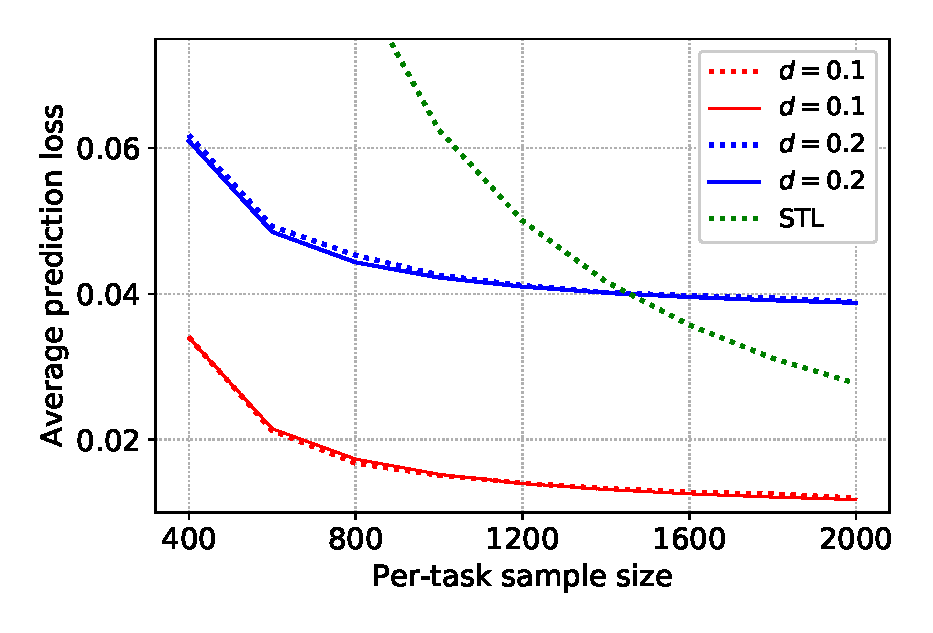
\includegraphics[width=0.98\textwidth]{figures/same_covariates.eps}
		\caption{Example \ref{ex_same_cov}}
		\label{fig_same_cov}
	\end{subfigure}\hfill
	\begin{subfigure}[b]{0.33\textwidth}
		\centering
		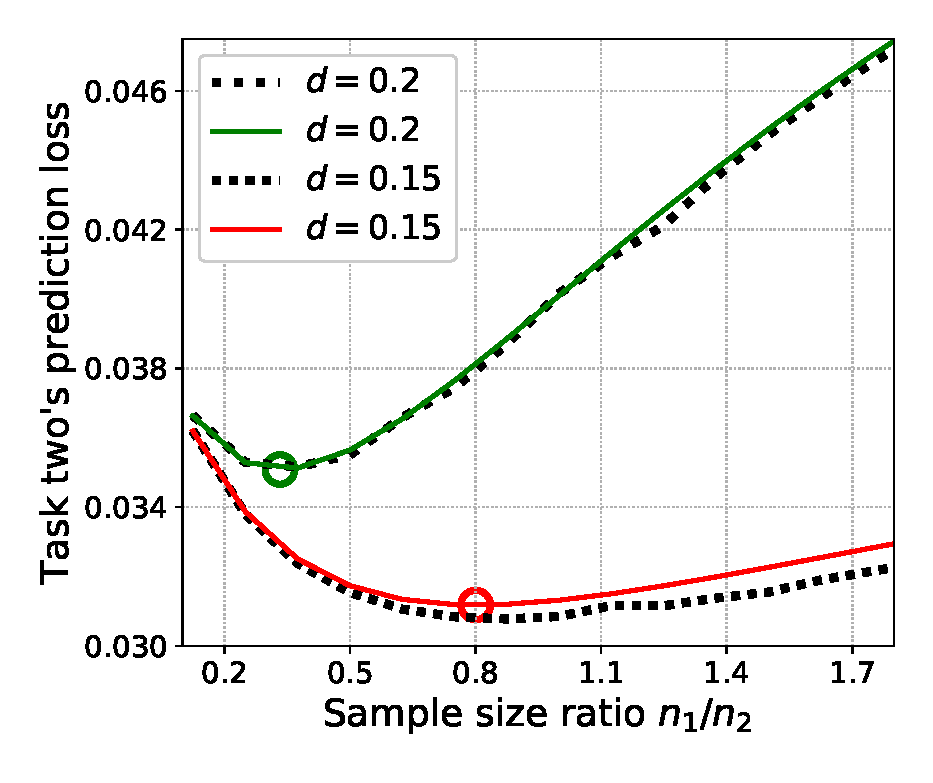
\includegraphics[width=0.98\textwidth]{figures/sample_ratio_several_d.eps}
		\caption{Example \ref{ex_sample_ratio}}
		\label{fig_size}
	\end{subfigure}\hfill
	\begin{subfigure}[b]{0.33\textwidth}
		\centering
		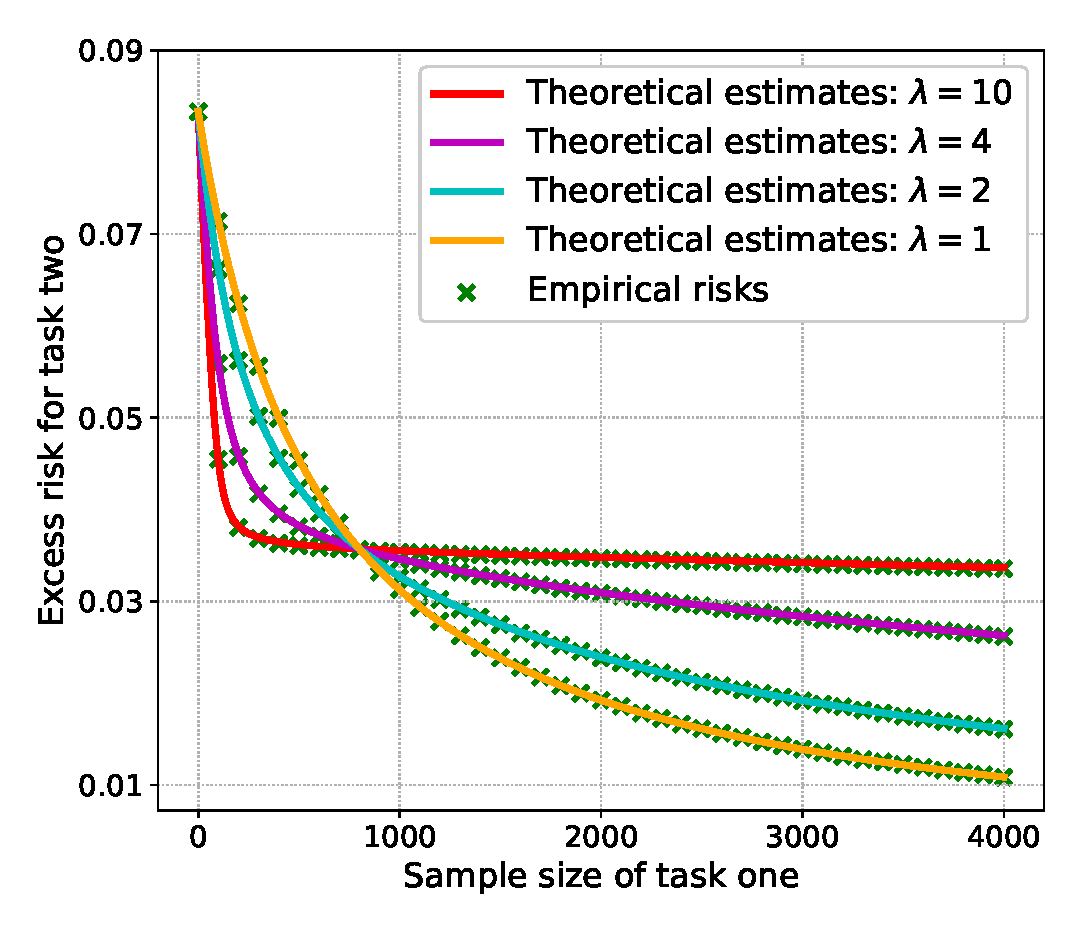
\includegraphics[width=0.98\textwidth]{figures/covariate_shift.eps}
		\caption{Example \ref{ex_covshift}}
		\label{fig_covariate}
	\end{subfigure}
	\caption{%Three takeaways of our theory in Section \ref{sec_insight}.
	Our estimated losses (solid line) match the empirical losses (dotted line) accurately under various settings in dimension $p = 200$.
	\textbf{Left.} Validating Example \ref{ex_same_cov} for ten tasks: the noise variance $\sigma^2$ is $1/4$.
	\textbf{Middle.} Validating Example \ref{ex_sample_ratio} for two tasks: we discover an interesting phenomena by fixing task two's sample size and increasing task one's sample size.
	Moreover, our result accurately predicts the critical point (marked in circle) of the loss curve.
%	Depending on how large the distance $d^2$ is, task two's prediction loss decreases initially before increasing again, or decreases monotonically.
	\textbf{Right.} We show how different levels of covariate shift affect hard parameter sharing when there is no bias.
	Having covariate shift increases task two's prediction loss when task two's sample size is smaller than task one. Otherwise, having covariate shift (surprisingly) decreases task two's prediction loss.}
	\label{fig_model_shift_phasetrans}
\end{figure*}



\paragraph{Sample efficiency.}
First, we validate the result of Example \ref{ex_same_cov}.
Figure \ref{fig_same_cov} shows the average prediction loss over ten tasks as we increase the number of samples per-task from $400$ to $2000$.
In all the parameter settings, our results estimate the empirical losses accurately.
We also observe a trend that the average prediction loss increases as we increase distance $d$ from $0.1$ to $0.2$.
Our work explains the differences between these two settings since $d^2 = 0.1^2$ is always smaller than $\frac{\sigma^2 p}{n - p}$, but $d^2 = 0.2^2$ is not.
%Second, when $d = 0.1$, we have that $d^2 \le \frac{\sigma^2 p}{n - p}$ for all values of $n$, hence the average prediction loss of hard parameter sharing is always lower than STL.
Indeed, we observe a crossover point between hard parameter sharing and STL.
Finally, for $d = 0.2$, looking horizontally, we find that HPS requires fewer samples per-task than STL to achieve the same loss level. %\FY{I do not quite understand this sentence about "3x fewer", because how much data needed depends on $d$ and the prediction loss level we are looking at. For example, at the cross point, this ratio is 1. }

\paragraph{Sample size ratio.}
Second, we validate the result of Example \ref{ex_sample_ratio}.
Figure \ref{fig_size} shows task two's prediction loss  as we increase the sample ratio $n_1 / n_2$ from $1/10$ to $7/10$.
%Again, our estimates are accurate compared to the empirical losses.
We consider a regime where task two consists of $80,000$ samples, and task one's sample size varies from $8,000$ to $56,000$. 
The task-specific variance (which scales with model distance) is $d = 0.2$, the noise variance is $\sigma^2 = 4^2$, and the shared signal variance is $1$. We observe that as we increase the sample ratio, task two's prediction loss decreases initially but later will increase when the sample ratio is above a certain level.
On the other hand, when $d = 0.15$, task two's prediction loss decreases faster.
Intuitively, this is because bias increases less for smaller $d^2$.
%Our result from Corollary \ref{cor_MTL_loss} explains this trend.

\paragraph{Covariate shift.}
Finally, we validate the result of Example \ref{ex_covshift}.
Figure \ref{fig_covariate} shows task two's prediction loss as we increase task one's sample size.
Recall that $\lambda$ measures the severity of covariate shifts---a larger $\lambda$ means a larger covariate shift.
We indeed observe the dichotomy in Example \ref{ex_covshift} at $n_1 = 800$.
The sample size $n_2$ is $800$ and the noise variance $\sigma^2$ is $1/4$.
%Covariate shift: We set $\kappa = 1$ and $d = 0$.
%We set $\rho_2 = 4$ and vary $\rho_1$ from $5$ to $25$ for sample sizes.
%We use the scale parameter $\lambda = 1$ for the curve without covariate shift and $\lambda = 2$ for the curve with covariate shift (cf. Section \ref{sec_covshift}).


%Recall that Section \ref{sec_data_size} shows that increasing the data size of the source task does not always improve the performance of MTL for the target task.
%In Figure \ref{fig_ab_data}, we show that for source task MR and target task SST, there is a transition from positive to negative transfer as we increase the data size of the source task.
%Our result provides a fine-grained insight on the covariance alignment algorithm proposed in \cite{WZR20}.
%Recall that the covariance alignment procedure in \cite{WZR20} adds an additional module between the word embedding representation and the shared module.
%When the source task data size is particularly large compared to the target task, we show that applying the covariance alignment algorithm results in more significant gains.
%In Figure \ref{fig_ab_cov}, we observe that the benefit from aligning task covariances becomes more significant for LSTM and MLP as we increase the number of datapoints of the source task.

%\begin{table}
%	\begin{center}
%		\begin{tabular}{c c c c c}
%			\toprule
%			\multirow{2}{*}{{\bf Models}} & \multicolumn{2}{c}{\begin{minipage}{1.1in}\begin{center}
%				                                                                          MR, SST, SUBJ, CR, MPQA, TREC\end{center}\end{minipage}} & \multicolumn{2}{c}{\begin{minipage}{1.1in}\begin{center}MR, SST, SUBJ, CR, MPQA\end{center}\end{minipage}} \\
%			\cmidrule(lr){2-3} \cmidrule(lr){4-5}
%			& {\bf Stanford} & {\bf Alignment} & {\bf Stanford} & {\bf Alignment} \\
%			\midrule
%			{\bf MLP}  & > 100\% & 39\% & 25\% & 25\% \\
%			{\bf LSTM} & 36\% & 36\% & 28\% & 25\% \\
			% {\bf CNN}  & 76\% & - & 32\% & -\\
%			\bottomrule
%		\end{tabular}
%	\end{center}
%	\caption{Taskonomy experiment.}
%	\label{tab:taskonomy}
%\end{table}
%\begin{figure}[!t]
%	\centering
%	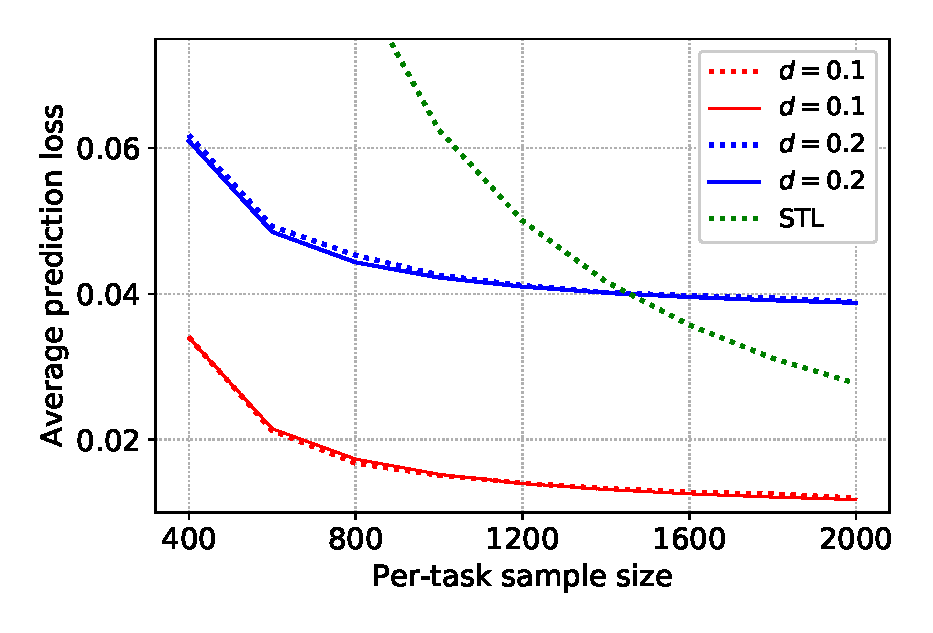
\includegraphics[width=0.35\textwidth]{figures/same_covariates.eps}
%	\caption{Validating Example \ref{ex_same_cov} in Section \ref{sec_same} for $10$ tasks: our estimated loss (solid line) matches the empirical loss (dotted line) accurately for various task-specific variance $d^2$ and sample size $n$ settings. The feature dimension $p$ is $200$, and noise variance $\sigma^2$ is $1/4$.}
%	\label{fig_same_cov}
%\end{figure}

\subsection{Further Studies on Text Classification Tasks}\label{sec_text}

Our results and simulations are all in the high-dimensional linear regression setting.
How well do they extend to other scenarios?
In this section, we conduct further studies on six text classification datasets.
Our datasets include a movie review sentiment dataset (MR) \cite{pang2005seeing}, a sentence subjectivity dataset (SUBJ) \cite{pang2004sentimental}, a customer reviews dataset (CR) \cite{hu2004mining}, a question type dataset (TREC) \cite{li2002learning}, an opinion polarity dataset (MPQA) \cite{wiebe2005annotating}, and the Stanford sentiment treebank (SST) dataset \cite{socher2013recursive}.
%The question is to predict positive or negative sentiment expressed in the text.
Our model consists of a word embedding layer with GloVe embeddings \cite{pennington2014glove} followed by a long-short term memory (LSTM) or a multi-layer perception (MLP) layer \cite{lei2018simple}.\footnote{For MLP, we apply an average pooling layer over word embeddings. For LSTM, we add a shared feature representation layer on top of word embeddings.}

%multi-layer perceptron (MLP), LSTM, CNN on all tasks
%We use this task to verify our theoretical results on model capacity and task covariance in real world.
%{\it ChestX-ray14.} This dataset contains 112,120 frontal-view X-ray images \cite{chexnet17}.
%There are 14 diseases (tasks) for every image that we would like to predict.
%We use densenet121 as the shared module \cite{huang2017densely}.
%We treat each label as one task a binary classification problem and formulate it as a 14-task multi-task learning problem.
%This dataset is curated where the labels
%We use the CheXNet model from~\cite{chexnet}, which is a 121-layer convolutional neural network on all tasks.
%For the text classification experiment, we encode each word using the GLoVe word embeddings.%
%\footnote{http://nlp.stanford.edu/data/wordvecs/glove.6B.zip}
%We evaluate three model choices.
%\textit{Predicting transfer effect via STL results.}
%We show that the single-task based metric proposed in Section \ref{sec_similarity} can predict positive or negative transfer in MTL.
%A common challenge in the study of MTL is that the results can be hard to understand.
%It is difficult to predict when MTL performs well without running extensive trials.
%Our insight is that we can use STL results to help understand MTL results.
%Table \ref{tab:mtl_better_than_stl} shows the result on both the sentiment analysis and the ChestX-ray14 tasks.
%We find that using a threshold of $\tau = 0.1$, the STL results correctly predict positive or negative transfer with $75.6\%$ precision and $38.8\%$ recall among $30$ times $5$ (random seeds) task pairs!
%We observe similar results for $91$ task pairs from the ChestX-ray14 dataset.
%The results show that STL results are indicative of MTL results.

\paragraph{Sample size ratio.}
First, we we show that our observation in Figure \ref{fig_size} also occurs in the text classification tasks.
In Figure \ref{fig_ab_data}, we observe that for multiple example task pairs, increasing task one's sample size improves task two's prediction accuracy initially, but hurts eventually.
On the $y$-axis, we plot task two's test accuracy using HPS, subtracted by its STL test accuracy.
%validate that as we increase the sample ratio while keeping task two's sample size fixed, task two's prediction accuracy does not always increase.
We fix task two's sample size at $1000$ and increase task one's sample size from $100$ to $3000$.

These examples and the one in Figure \ref{fig_size} suggest a natural progressive training schedule, where we add samples progressively until performance drops.
Concretely, here is one implementation of this idea.
%In particular, Figure \ref{fig_size} (and our analysis) shows that $L(\hat{\beta}_t^{\MTL})$ behaves as a quadratic function over $\rho_1$.
%More generally, depending on how large $\Psi(\beta_1, \beta_2)$ is, $L(\hat{\beta}_t^{\MTL})$ may also be monotonically increasing or decreasing.
%Based on this observation, we propose a progressive training schedule to improve the compuational efficiency of hard parameter sharing.
\begin{itemize}
	\item We divide the training data into $S$ batches.
	We divide the training procedure into $S$ stages. During every stage, we progressively add one more data batch.
	\item During every stage, we train for $T$ epochs using only the $S$ batches. If the validation accuracy drops compared to the previous round's result or reach a desired threshold $\tau$, we terminate.
%	Algorithm \ref{alg_inc_train} in Appendix \ref{app_experiments} describes the procedure in detail.
\end{itemize}
If we apply this procedure to the settings of Figure \ref{fig_ab_data} and \ref{fig_size}, it will terminate once reaching the optimal sample ratio.
%See Algorithm \ref{alg_inc_train} for a complete description for two tasks.
The advantage of this procedure is that it reduces the computational cost compared to standard round-robin training schedules.
For example, if the procedure terminates at 30\% of all batches, then SGD only passes over 30\% of its data, whereas standard round-robin training passes over 100\% of task one's data.


%We fill in the details of the experimental procedure used for the results in Figure \ref{fig_ablation}.
%\squishlist
%	\item Task similarity: We select a similar and a dissimilar source task compared to the target task using domain knowledge.
%First pair: the customer review dataset (CR) , which predicts whether a review is positive or negative, is more similar to SST (sentiment treebank) than MPQA (question type).
%Second pair: SST is more similar to MR since they both concern about positive or negative opinions expressed the text.
%TREC is less similar to MR because the task is about question types.
%Third pair: MPQA (opinion polarity) is more similar to TREC (question type)
We evaluate the progressive training procedure on the six text classification datasets.
First, we conduct multi-task training over all $15$ two-task pairs from the six datasets.
We focus on task two's test accuracy and set $\tau$ as task two's test accuracy obtained via the standard round-robin training schedule.
We include all of task two's data and progressively add task one's data using the procedure described above.
Since the prediction accuracy has been controlled the same, we compare the computational cost.
We find that when averaged over all $15$ two-task pairs, this procedure requires only $45\%$ of the computational cost to reach the desired accuracy $\tau$ for task two.
%Our insight is that since adding more samples from the source task does not always help, we can improve efficiency by adding source samples \textit{progressively} during training.
%\textbf{Improving transfer learning training efficiency.}
%We show that Algorithm \ref{alg_inc_train} also applies to transfer learning settings.
%Compared to fine-tuning the source model on the target task, we show that our proposed method reduces the computional cost by \alert{$xx\%$}, without sacrificing accuracy.
Second, we conduct multi-task training on all six datasets jointly.
We extend our procedure to all six datasets. We include the data from all tasks except SST. For SST, we progressively add data similar to the above procedure.
We set $\tau$ to be the average test accuracy of all six tasks obtained using standard round-robin training.
We find that adding samples progressively from SST requires less than $35\%$ of the computational cost to reach the same average test accuracy $\tau$.
%As a further validation, excluding TREC, we observe similar comparative results.
%The data efficiency ratio of using MLP is $100\%$ because the average performance of MTL is worse than the average of STL.
%We further show that applying incremental training helps reduce the data efficiency ratio to \alert{$xx\%$}.
%If TREC is not included, we see that only $25\%$ of the labeled data is needed.



%	\begin{subfigure}[b]{0.33\textwidth}
%		\centering
%		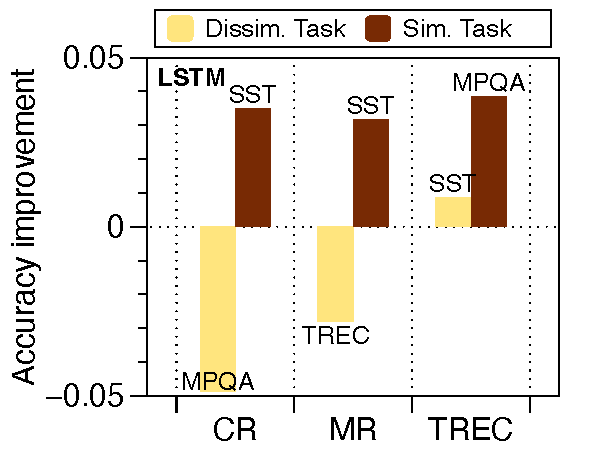
\includegraphics[width=0.975\textwidth]{figures/task_sim_norm_lstm.pdf}
%		\caption{Task similarity}
%		\label{fig_ab_sim}
%	\end{subfigure}%
%	\caption{Validating the three results of Section \ref{sec_insight} on sentiment analysis tasks. (a) Adding a semantically similar source task in MTL performs better than adding a dissimilar task.
%	(b) As source/target sample ratio increases, we observe a transition from positive to negative transfer.
%	(c)
%	Note: (S) denotes the source task and (T) denotes the target task.}


%\begin{minipage}[t]{.58\textwidth}
%	\vspace{-0.1in}
%	\centering
%  \begin{tabular}{c c c c c}
%	\toprule
%		\multirow{2}{*}{{\bf Threshold}}  & \multicolumn{2}{c}{{\bf Sentiment
%		analysis}} & \multicolumn{2}{c}{{\bf ChestX-ray14}} \\
%		& Precision &  Recall & Precision &  Recall \\
%		\cmidrule(lr){1-1} \cmidrule(lr){2-3} \cmidrule(lr){4-5}
%		0.0 & 0.596 & 1.000 & 0.593 & 1.000 \\
%		0.1 & \textbf{0.756} & \textbf{0.388} & \textbf{0.738} & \textbf{0.462} \\
%		0.2 & 0.919 & 0.065 & 0.875 & 0.044 \\
		% 0.3 & 1.000 & 0.004 &     - &     - \\
%	\bottomrule
%	\end{tabular}
%	\vspace{0.1in}
%	\captionof{table}{Single-task learning results can help predict postive or negative transfer in multi-task learning.}
%	\label{tab:mtl_better_than_stl}
%\end{minipage}%
%\quad


\paragraph{Covariate shift.}
Recall from Example \ref{ex_covshift} that having covariate shifts worsens the variance (hence the loss) of hard parameter sharing when the sample ratio increases.
This highlights the need for correcting covariate shifts when the sample size ratio rises.
To this end, we study a covariance alignment procedure proposed in \cite{WZR20}, designed to correct covariate shifts.
The idea is to add an alignment module between the input and the shared module $B$.
This module is then trained together with $B$ and the output layers. We refer to \cite{WZR20} for more details about the procedure and the implementation.
%We validate our insight on this procedure in the experiments.
%We implement the covariance alignment procedure following \cite{WZR20}.

We conduct multi-task training on all $15$ task pairs from the six datasets.
In Figure \ref{fig_ab_cov}, we measure the performance gains from performing covariance alignment vs. HPS.
To get a robust comparison, we average the improvements over the 15 task pairs.
The result shows that as the sample size ratio increases, performing covariance alignment provides more significant gains over HPS.
We fix task two's sample size at $1,000$, and increase task one's sample size from $1,000$ to $3,000$.

%\begin{figure}[!t]
%	\centering
%	\begin{subfigure}[b]{0.5\textwidth}
%		\centering
%		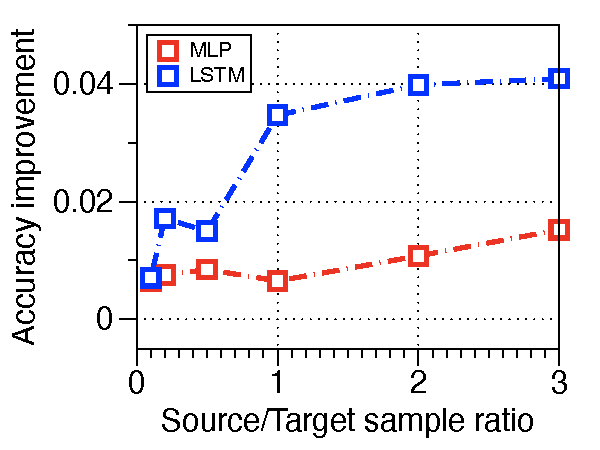
\includegraphics[width=0.5\textwidth]{figures/ratio_alignment_norm_diff_all.pdf}
%		\caption{Averaged over all 16 task pairs}
%		\label{fig_ab_cov}
%	\end{subfigure}\hfill
%	\begin{subfigure}[b]{0.5\textwidth}
%		\centering
%		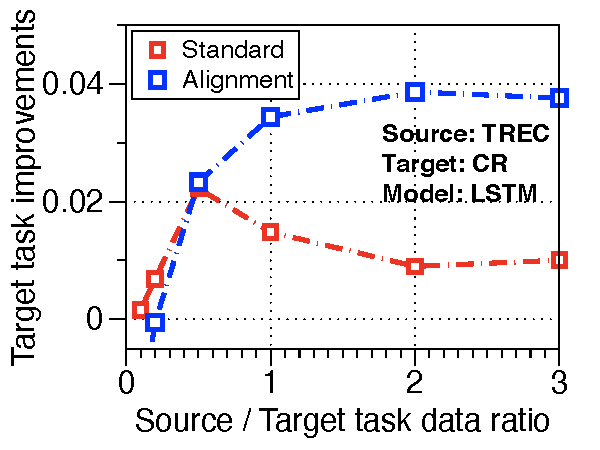
\includegraphics[width=0.5\textwidth]{figures/ratio_alignment_norm_trec_cr_lstm.pdf}
%		\caption{An example task pair}
%		\label{fig_cov_a}
%	\end{subfigure}
%	\caption{ (TREC and CR)}
%\end{figure}

%\textbf{Further results of the covariance alignment procedure.}
%Our results in Figure \ref{fig_ab_cov} are averaged over all the task pairs.
%In Figure \ref{fig_covariate_app}, we show two task pairs as examples.
%In Figure \ref{fig_cov_a}, we observe that for the particular task pair, covariance alignment provides more significant gains when the sample ratio is large.
%In Figure \ref{fig_cov_b}, we observe that covariance alignment does not always improve over the baseline multi-task learning model.
%One explanation is that MR and SST are similar tasks, hence adding the alignment module is unnecessary.
%An interesting question is to understand when adding the alignment module benefits the multi-task learning model.
%We leave this question for future work.
%Note: For text classification tasks, the source task training data size ranges from 500 to 1,500 and target task training data size is 1000; For ChestX-ray14,

%\begin{figure}[!h]
%	\centering
%	\begin{subfigure}[b]{0.48\textwidth}
%		\centering
%		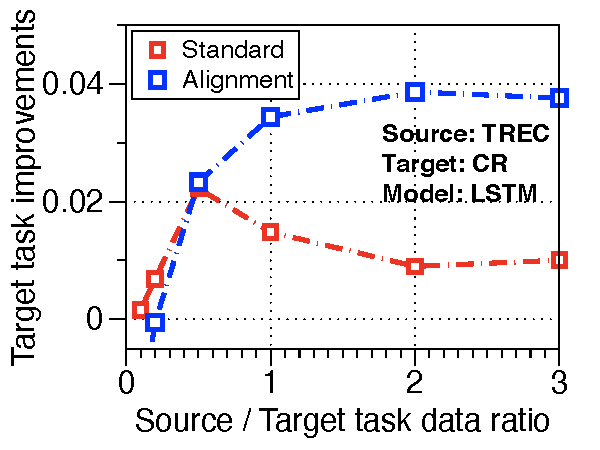
\includegraphics[width=0.7\textwidth]{figures/ratio_alignment_norm_trec_cr_lstm.pdf}
%		\caption{Task pair TREC and CR}
%		\label{fig_cov_a}
%	\end{subfigure}\hfill
%		\begin{subfigure}[b]{0.48\textwidth}
%		\centering
%		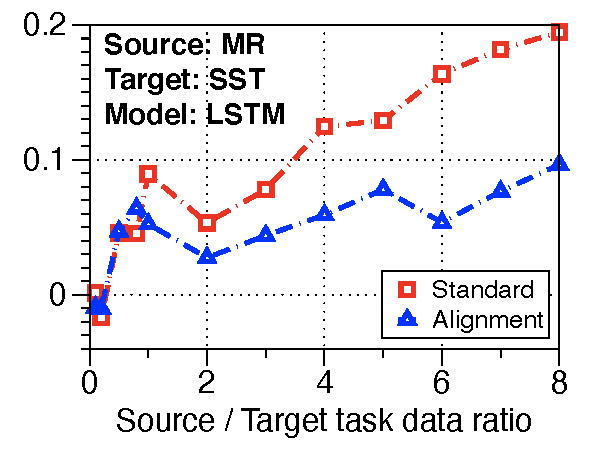
\includegraphics[width=0.7\textwidth]{figures/ratio_alignment_mr_sst_lstm.pdf}
%		\caption{Task pair MR and SST}
%			\label{fig_cov_b}
%	\end{subfigure}
%	\caption{(a) For the task pair TREC and CR, adding the covariance alignment procedure provides more improvement when the source/target sample ratio is large.
%	(b) For the task pair MR and SST, adding the covariance alignment procedure hurts performance.
%	One explanation is that MR and SST are similar tasks, hence adding the alignment module is unnecessary.}
%	\label{fig_covariate_app}
%\end{figure}


\begin{figure}%[!t]
	\begin{subfigure}[t]{0.5\textwidth}
		\centering
		\vspace{0pt}
		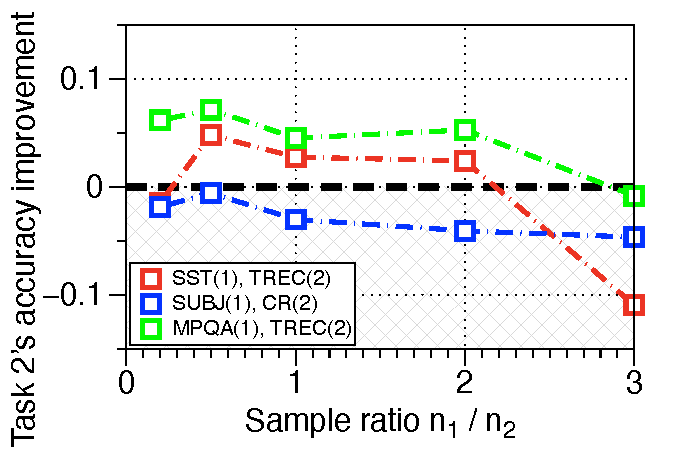
\includegraphics[width=0.8\textwidth]{figures/fig3a.pdf}
		\caption{HPS vs. STL}
		\label{fig_ab_data}
	\end{subfigure}\hfill
	\begin{subfigure}[t]{0.5\textwidth}
		\centering
		\vspace{0pt}
		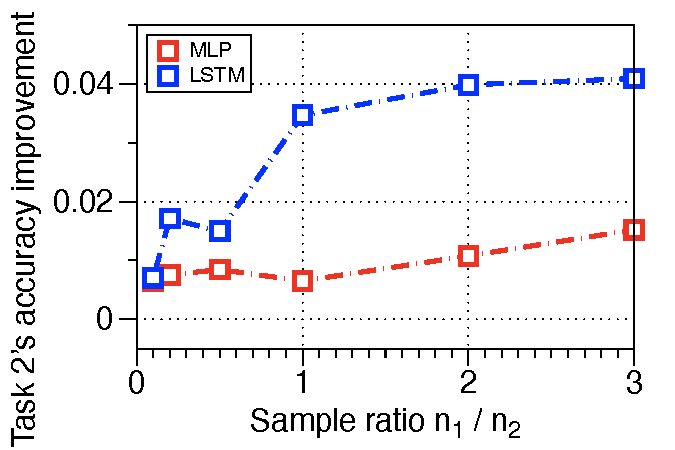
\includegraphics[width=0.8\textwidth]{figures/fig3b.pdf}
		\caption{HPS vs. covariance alignment}
		\label{fig_ab_cov}
	\end{subfigure}
	\caption{Comparing hard parameter sharing (HPS) to single-task learning (STL) and a covariance alignment approach proposed by \cite{WZR20}:
	In Figure \ref{fig_ab_data}, we observe that for multiple task pairs, increasing task one's sample size improves task two's prediction accuracy initially, but hurts eventually -- a phenomenon similar  to Figure \ref{fig_size}.
	In Figure \ref{fig_ab_cov}, we observe that as task one's sample size increases, covariance alignment improves more over HPS.}
	\label{fig_text}
%	\begin{minipage}[t]{0.4\textwidth}
%		\centering
%		\vspace{0pt}
%		\begin{tabular}{c c c}
%		\toprule
		% \multirow{2}{*}{{\bf Models}} & \multicolumn{2}{c}{\begin{minipage}{1.2in}\begin{center}
		% Sentiment\\ analysis\end{center}\end{minipage}} \\
%		\multirow{2}{*}{{\bf Models}} & \multicolumn{2}{c}{\bf Sentiment analysis} \\
		% \cmidrule(lr){2-3}
%		& all tasks & w/o TREC \\
%		\midrule
%		{\bf MLP}  & 31\% & 29\% \\
%		{\bf LSTM} & 35\% & 34\% \\
%		{\bf CNN}  & 30\% & 28\% \\
%		\bottomrule
%		\end{tabular}
%		\captionof{table}{Finding the best sample ratio via a progressive training schedule.}
%		\label{tab:taskonomy}
%	\end{minipage}
\end{figure}

%\begin{algorithm}[!t]
%	\caption{A progressive training schedule given two tasks}
%	\label{alg_inc_train}
%	\begin{algorithmic}[1]
%		\Input Two tasks $(X^{(1)}, Y^{(1)})$ and $(X^{(2)}, Y^{(2)})$.
%		\Param A shared module $B$, output layers $A_1, A_2$ as in the hard parameter sharing architecture.
%		\Req \# batches $S$, epochs $T$, task $2$'s validation accuracy $\hat{g}(B; W_2)$, a threshold $\tau\in(0,1)$.
%		\Output The trained modules $B, A_2$ optimized for task $2$.
%		\State Divide $(X^{(1)}, Y^{(1)})$ randomly into $S$ batches: $(x^{(1)}, y^{(1)}), \dots, (x^{(S)}, y^{(S)})$.
%		\For{$i = 1,\dots, S$}
%			\For{$j = 1,\dots, T$}
%				\State Update $B, A_1, A_2$ using the training data $\set{x^{(k)}, x^{(k)}}_{k=1}^i$ and  $(X^{(2)}, Y^{(2)})$.
%			\EndFor
%			\State Let $a_i = \hat{g}(B; A_2)$ be the validation accuracy.
%			\If{$a_i < a_{i-1}$ or $a_i > \tau$}
%				\State \textbf{break}
%			\EndIf
%		\EndFor
%	\end{algorithmic}
%\end{algorithm}

\iffalse
\section{Conclusions and Discussions}\label{sec_conclude}

This work studied generalization properties of a widely used hard parameter sharing approach for multi-task learning.
We provided sharp bias-variance tradeoffs of HPS in high-dimensional linear regression.
Using these results, we analyzed how varying sample sizes and covariate shifts impact HPS, and rigorously explained several empirical phenomena such as negative transfer and covariate shift related to these dataset properties.
We validated our theory and conducted further studies on text classification tasks.
We describe several open questions for future work.
%First, it would be interesting to tighten our estimate in Corollary \ref{cor_MTL_loss}, which would extend the observation in Figure \ref{fig_size} to small $n_1$.
%Second, it would be interesting to extend our result to classification problems such as logistic regression.
First, our result in Corollary \ref{cor_MTL_loss} involves an error term that scales down with $n_1$.
Tightening this error bound requires showing the limit of $\normFro{({Z^{(1)}}^{\top} Z^{(1)} + {Z^{(2)}}^{\top} Z^{(2)})^{-1} {Z^{(1)}}^{\top} Z^{(1)}}^2$ for two isotropic sample covariance matrices.
This requires studying the asymptotic singular values distribution of the non-symmetric matrix $({Z^{(1)}}^{\top} Z^{(1)})^{-1}{Z^{(2)}}^{\top} Z^{(2)}+\id$, which is still an open problem in random matrix theory.
%FY: $+\id$ is very important and makes the problem very hard; otherwise the problem can be solved with current RMT methods.
The eigenvalue distribution of this matrix, which has been obtained in \cite{Fmatrix}, might be helpful towards resolving this problem.
%but its singular values will follow a different distribution since the matrix is not symmetric.
 %might require new techniques beyond the current ones in random matrix theory .%\HZ{to add}.
Second, it would be interesting to extend our results to classification problems.
Several recent work have made remarkable progress for logistic regression in the high-dimensional setting, e.g. \cite{sur2019modern}.
An interesting question is to study logistic regression in a multiple-sample setting.
\fi

% \section*{Acknowledgements}
%Thanks to Edgar Dobriban, Vaggos Chatziafratis, Mayee Chen, and Ruoxuan Xiong for helpful discussions at various stages of this work. Hongyang R. Zhang and Weijie J. Su's contributions were in part supported by the Wharton Dean's Fund for Postdoctoral Research.
%We gratefully acknowledge the support of DARPA under Nos. FA86501827865 (SDH) and FA86501827882 (ASED); NIH under No. U54EB020405 (Mobilize), NSF under Nos. CCF1763315 (Beyond Sparsity), CCF1563078 (Volume to Velocity), and 1937301 (RTML); ONR under No. N000141712266 (Unifying Weak Supervision); the Moore Foundation, NXP, Xilinx, LETI-CEA, Intel, IBM, Microsoft, NEC, Toshiba, TSMC, ARM, Hitachi, BASF, Accenture, Ericsson, Qualcomm, Analog Devices, the Okawa Foundation, American Family Insurance, Google Cloud, Swiss Re, the HAI-AWS Cloud Credits for Research program, and members of the Stanford DAWN project: Teradata, Facebook, Google, Ant Financial, NEC, VMWare, and Infosys. The U.S. Government is authorized to reproduce and distribute reprints for Governmental purposes notwithstanding any copyright notation thereon. Any opinions, findings, and conclusions or recommendations expressed in this material are those of the authors and do not necessarily reflect the views, policies, or endorsements, either expressed or implied, of DARPA, NIH, ONR, or the U.S. Government.


%%%%%%%%%%%%%%%%%%%%%%%%%%%%%%%%%%%%%%%%%%%%%%
%% Supplementary Material, if any, should   %%
%% be provided in {supplement} environment  %%
%% with title and short description.        %%
%%%%%%%%%%%%%%%%%%%%%%%%%%%%%%%%%%%%%%%%%%%%%%
\begin{supplement}
\textbf{Supplement to ``Hard Parameter Sharing in High-dimensional Linear Regression"}.
In \cite{MTL_suppl}, we provide the proofs of the technical results in Sections \ref{sec_HPS}-\ref{sec_diff}, including Lemma \ref{lem_HPS_loss}, Theorem \ref{thm_many_tasks}, Theorem \ref{cor_MTL_loss}, Proposition \ref{lem_hat_v}, Theorem \ref{thm_main_RMT} and Proposition \ref{prop_main_RMT}. 
%and give the technical proofs of the main theorems, Theorems \ref{thm_regularbm}, \ref{thm_twgram}, \ref{thm_twgraph} and  \ref{thm_twgraph_sparse}.
\end{supplement}


%%%%%%%%%%%%%%%%%%%%%%%%%%%%%%%%%%%%%%%%%%%%%%%%%%%%%%%%%%%%%
%%                  The Bibliography                       %%
%%                                                         %%
%%  imsart-???.bst  will be used to                        %%
%%  create a .BBL file for submission.                     %%
%%                                                         %%
%%  Note that the displayed Bibliography will not          %%
%%  necessarily be rendered by Latex exactly as specified  %%
%%  in the online Instructions for Authors.                %%
%%                                                         %%
%%  MR numbers will be added by VTeX.                      %%
%%                                                         %%
%%  Use \cite{...} to cite references in text.             %%
%%                                                         %%
%%%%%%%%%%%%%%%%%%%%%%%%%%%%%%%%%%%%%%%%%%%%%%%%%%%%%%%%%%%%%

%% if your bibliography is in bibtex format, uncomment commands:
\bibliographystyle{imsart-number}
%\bibliographystyle{imsart-nameyear}

%\bibliographystyle{abbrv}
%\bibliographystyle{plain}
\bibliography{rf,ref_mtl}
 % Style BST file (imsart-number.bst or imsart-nameyear.bst)
%\bibliography{bibliography}       % Bibliography file (usually '*.bib')



%% or include bibliography directly:
%\begin{thebibliography}{4}
%%%
%\bibitem{r1}
%\textsc{Billingsley, P.} (1999). \textit{Convergence of
%Probability Measures}, 2nd ed.
%Wiley, New York.
%
%\bibitem{r2}
%\textsc{Bourbaki, N.}  (1966). \textit{General Topology}  \textbf{1}.
%Addison--Wesley, Reading, MA.
%
%\bibitem{r3}
%\textsc{Ethier, S. N.} and \textsc{Kurtz, T. G.} (1985).
%\textit{Markov Processes: Characterization and Convergence}.
%Wiley, New York.
%
%\bibitem{r4}
%\textsc{Prokhorov, Yu.} (1956).
%Convergence of random processes and limit theorems in probability
%theory. \textit{Theory  Probab.  Appl.}
%\textbf{1} 157--214.
%\end{thebibliography}

\end{document}
